\documentclass[12pt]{article}\usepackage[]{graphicx}\usepackage[]{color}
%% maxwidth is the original width if it is less than linewidth
%% otherwise use linewidth (to make sure the graphics do not exceed the margin)
\makeatletter
\def\maxwidth{ %
  \ifdim\Gin@nat@width>\linewidth
    \linewidth
  \else
    \Gin@nat@width
  \fi
}
\makeatother

\definecolor{fgcolor}{rgb}{0.345, 0.345, 0.345}
\newcommand{\hlnum}[1]{\textcolor[rgb]{0.686,0.059,0.569}{#1}}%
\newcommand{\hlstr}[1]{\textcolor[rgb]{0.192,0.494,0.8}{#1}}%
\newcommand{\hlcom}[1]{\textcolor[rgb]{0.678,0.584,0.686}{\textit{#1}}}%
\newcommand{\hlopt}[1]{\textcolor[rgb]{0,0,0}{#1}}%
\newcommand{\hlstd}[1]{\textcolor[rgb]{0.345,0.345,0.345}{#1}}%
\newcommand{\hlkwa}[1]{\textcolor[rgb]{0.161,0.373,0.58}{\textbf{#1}}}%
\newcommand{\hlkwb}[1]{\textcolor[rgb]{0.69,0.353,0.396}{#1}}%
\newcommand{\hlkwc}[1]{\textcolor[rgb]{0.333,0.667,0.333}{#1}}%
\newcommand{\hlkwd}[1]{\textcolor[rgb]{0.737,0.353,0.396}{\textbf{#1}}}%
\let\hlipl\hlkwb

\usepackage{framed}
\makeatletter
\newenvironment{kframe}{%
 \def\at@end@of@kframe{}%
 \ifinner\ifhmode%
  \def\at@end@of@kframe{\end{minipage}}%
  \begin{minipage}{\columnwidth}%
 \fi\fi%
 \def\FrameCommand##1{\hskip\@totalleftmargin \hskip-\fboxsep
 \colorbox{shadecolor}{##1}\hskip-\fboxsep
     % There is no \\@totalrightmargin, so:
     \hskip-\linewidth \hskip-\@totalleftmargin \hskip\columnwidth}%
 \MakeFramed {\advance\hsize-\width
   \@totalleftmargin\z@ \linewidth\hsize
   \@setminipage}}%
 {\par\unskip\endMakeFramed%
 \at@end@of@kframe}
\makeatother

\definecolor{shadecolor}{rgb}{.97, .97, .97}
\definecolor{messagecolor}{rgb}{0, 0, 0}
\definecolor{warningcolor}{rgb}{1, 0, 1}
\definecolor{errorcolor}{rgb}{1, 0, 0}
\newenvironment{knitrout}{}{} % an empty environment to be redefined in TeX

\usepackage{alltt}
\usepackage{amsmath,lsalike,units,ifthen,tikz,graphicx,float}
\usepackage{rotating} 
\usepackage{enumitem}
\usepackage[T1]{fontenc}
\usepackage[utf8]{inputenc}
%\usepackage{draftwatermark}
\usetikzlibrary{calc}
\usetikzlibrary{automata, positioning}


%Watermark
%\SetWatermarkText{DRAFT}
%\SetWatermarkScale{10}
%probability operator
\newcommand{\p}{{\operatorname{p}}}
\newcommand{\s}{Swahili}
\newcommand{\pr}{productivity}
\newcommand{\ling}{lingusitic}
\newcommand{\li}{likelihood}
\newcommand{\nc}{noun class}
%equation number; no math; no label
%equation number; no math; no label
\newcommand{\eq}[1]{\bigskip\par
\stepcounter{equation}
\noindent\parbox{.5in}{(\theequation)}
\begin{minipage}[t]{4.5in}
#1
\end{minipage}
\par\bigskip}

%equation number; no math; with label
\newcommand{\eqlab}[2]{\bigskip\par
\refstepcounter{equation}
\noindent\parbox{.5in}{(\theequation)}
\label{#1}
\begin{minipage}[t]{4.5in}
#2
\end{minipage}
\par\bigskip}

\title{Morphological Use in Swahili}
%\author{Nick Kloehn \& Michael Hammond \\
%U.\ of Arizona}
\author{}
\date{}
\IfFileExists{upquote.sty}{\usepackage{upquote}}{}
\begin{document}

\maketitle
%Intro 
\section*{Morphological Productivity in Swahili}

%Here, I'm going to summarize the aims of this paper, and eventually describe the major claims.

%I'll hold off on this until later on. Do I need to focus on Gender to make this better?
%What would a gender paper look like? Well, Gender in Swahili is complicated.
%First, I need to look at Swahili morphology.

%I'll add some of what I've done and I'll do some more work on facts about the language, maybe add some lexico-statistics. I also have the wikipedia corpus. There will be a lot of paradigms here, but I can focus on what's important.

% Let's count the number of nouns in the language and what gender each noun is.

%Second, I need to look at Productivity.

%This will be tricky. I need to know all the literature. This is my week point. Summarize different perspectives of morphology, and discuss the claims. 

%Third, I need to show what I've done and why.

%Fourth, I need to show what it means.


Below is a basic summary of open categories in Swahili
% latex table generated in R 3.3.1 by xtable 1.8-2 package
% Mon Aug 28 14:15:14 2017
\begin{table}[ht]
\centering
\begin{tabular}{lrr}
  \hline
Category & Frequency & Frequency (per million) \\ 
  \hline
Adjectives & 905034 & 65768.10 \\ 
  Verbs & 2881258 & 209378.72 \\ 
  Nouns & 3991124 & 290031.79 \\ 
   \hline
\end{tabular}
\end{table}


% latex table generated in R 3.3.1 by xtable 1.8-2 package
% Mon Aug 28 14:15:14 2017
\begin{table}[ht]
\centering
\begin{tabular}{lrr}
  \hline
Category & Frequency & Frequency (per million) \\ 
  \hline
Nouns & 3991124 & 290031.79 \\ 
  Nouns derived from Adjectives & 28828 & 2094.91 \\ 
  Nouns derived from Verbs & 605476 & 43999.46 \\ 
   \hline
\end{tabular}
\end{table}


\begin{figure}
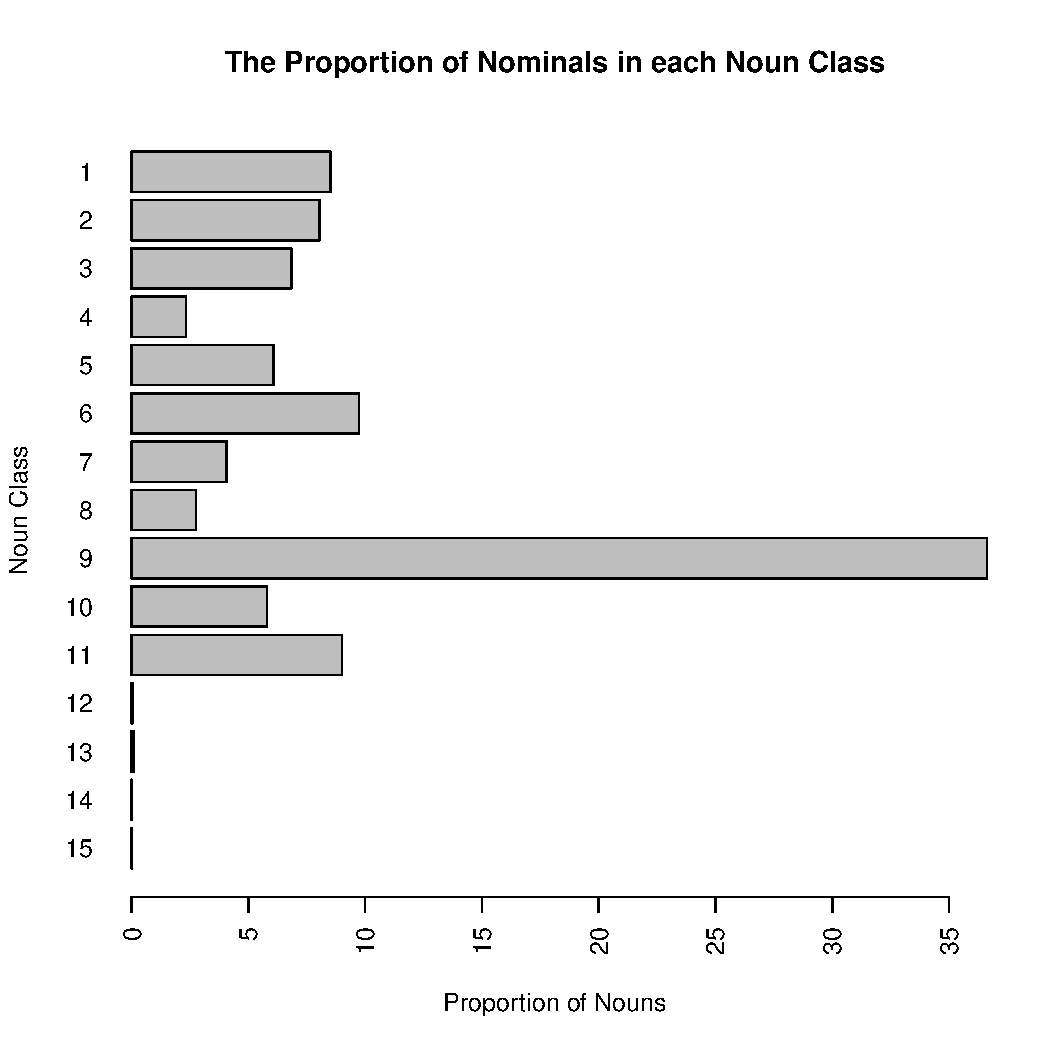
\includegraphics[width=\maxwidth]{figure/Lexicostats3-1} \end{figure}


The aim of this chapter is to isolate the predictors of novel word formation for words containing a given affix. In the past, it has been argued that parsibility and therefore productivity can be predicted by comparing the relationship between the log frequencies of all types of a given affix to the log frequencies of their affixless counterparts \cite{hay02}. Here, productivity occurs when for a given affix, the majority of affixless forms occur more frequently than their affixed counterparts. This measure of productivity has also been said to correlate with the number of hapaxes of a given type, which itself has been argued to correlate with productivity \cite{baay92}. Although our main interest is to understand the parameters of nominal classification, this section will also investigate novel word formation in both verbal and nominal affixes for both inflectional and derivational flavors. Increasing the empirical coverage of this comparison will allow us to ground one of the central questions of this investigation. This question has to do with an important typological aspect of Swahili morphology. Whereas languages like English and Dutch allow affixless forms of words, inflectional classes in Swahili require the existence of some affix at all times. Here, we will test and compare the prevalance of this type of affix with stems containing derivational classes, which may occur without some affix. In simple terms, for many Swahili affixes, there is no such thing as an affixless or non-derived forms, altering the forumlation of the ratio such that all inflectional morphemes will have un-derived frequencies of zeros. Here the model in it's current form would predict that no inflectional form should be parsible and therefore productive, although we  know this not to be the case. On the contrary, inflectional forms should nearly always be productive. To get around this we will work with the hypothesis that for these affixes, the frequency of morphological competitors (known as the cumulative root frequency \cite{cole89}) is key in predicting productivity of affixes of this type. This hypothesis implicitly alters our morphological model to suggest that productivity is not a result of discrimination between an affixed form and its affixless counterpart, but descrimination between an affix and all of its competitors of which the affixless form is just one possibility. If this parameter were true, we would be tempted to adopt a model of morphological systems that argue that descrimination is key in constructing paradigms \cite{blev2015}.

\noindent Here, we analyze the relationship between multiple standard methods of measuring affix productivity, and try to predict the existence of novel word forms of that affix. These measures of productivity are taken by analyzing the frequencies of word forms found in the Helsinki Corpus of Swahili, and then comparing them to novel forms found in the corpus using a k-folds method of cross validation. Simply, we subdivide the corpus into multiple parts and compare measures of morpheme productivity in one random subset to our dependent variable in another non-overlapping subset, k times. After establishing which measures are able to meaningfully predict productivty, we test this measure using twitter data extracted from a corpus of code-switched tweets.

\subsection{Methods}

We took 60 affixes of Swahili tagged in the Helsinki Corpus of Swahili of 13.2 million words. The corpus was accessed online via SSH, and frequency counts were extracted using a Python script. For each affix, we counted all types and their token frequency. Tokens in the corpus are tagged for both the affixed forms and the affixless lemmas and so we were able to automatically identify and count them. For each type, we then extracted the "affixless" forms by using a series of regular expressions. After extracting the bare forms, we then extracted the count of all variants of the form that did not include the original affixed form. Together, this allowed us to calculate the frequencies of all types of an affix, and their competative cumulative root frequencies.

\noindent This operation was performed on seven different random subsections of the corpus (of roughly 1.8 million words). For each subsection, we log transformed the frequency counts, and for each affix calculated how many types had a larger cumulative root frequency than affixed frequency. This number divided by the total type count gives us a ratio that should indicate the level of productivity. The higher the ratio, the more likely that that affix is to be productive. 

\noindent Next, we counted all the hapaxes of a given affix in a second random subset of the corpus. Essentially, we treat these counts as a measure of novel word formation. The idea here is that if an affix is productive, it should exhibit novel word formation. Furthermore, the working hypothesis is that more productive forms should exhibit a large number of novel words. So, if the type ratio is a predictor for productivity, then the ratio of the affix established in the previous subset should correlated with the number of hapaxes in the second subset.

\noindent Below are the affixes used in this study. There are four groups, which are divided by whether they occur nominally or verbally, and by whether they mark what we typically associate with inflectional, or derivational properties. These groups are not balanced, as they are unlikely to be in any language, but we've used the available tagsest developed by the creators of the corpus \cite{hcs}.

% These are all the types used
\begin{table}[t]
\caption{Verbal Extensions (Verbal Derivation Suffixes/Infixes)}

  % Morpheme Chart
  \begin{tabular}[t]{l|l|l|l}
  % Header with a lot of shortstacks
  \shortstack{\textbf{Morpheme}     \\  \textbf{Class}}       &
  \shortstack{\textbf{Form} \\ {\indent}}                                  & 
  \shortstack{\textbf{Grammatical} \\  \textbf{Distinction}}  & 
  \shortstack{\textbf{Example} \\ {\indent}}
  \\
  \hline
  % Body with all the morphemes tested
  \hline
  % Passive
  -(i/e)w-   &
  Infix &
  \textit{Passive} &
  \begin{tabular}[t]{lll} 
  pe- & -w- & -a  \\ 
  \textit{give} & \textsc{pass} & \textsc{fv}\\
  \multicolumn{3}{l}{'be given'}\\
  \end{tabular}\\
  \hline
   % Stative
  -(i/e)k-   &
  Infix  &
  \textit{Stative} &
  \begin{tabular}[t]{lll} 
  sik- & -ik- & -a  \\ 
  \textit{hear} & \textsc{stat} & \textsc{fv}\\
  \multicolumn{3}{l}{'be heard'}\\
  \end{tabular}\\
  \hline
     % Applicative
  \begin{tabular}{l}
  -(l)i- \\ -(l)e- 
  \end{tabular} &
  Infix  &
  \textit{Applicative} &
  \begin{tabular}[t]{lll} 
  pelek- & -e- & -a  \\
  \textit{send} & \textsc{appl} & \textsc{fv}\\
  \multicolumn{3}{l}{'send to'}\\
  \end{tabular}\\
  \hline
  % Causative
  \begin{tabular}{l}
    -(i/e)z- \\ -(i/e)sh-
  \end{tabular} &
  Infix &
  \textit{Causative} &
  \begin{tabular}[t]{lll} 
  ele- & -z- & -a  \\ 
  \textit{be clear} & \textsc{caus} & \textsc{fv}\\
  \multicolumn{3}{l}{'make clear'}\\
  \end{tabular}\\ 
  \hline
  % Reciprocal
  -an-   &
  Infix  &
  \textit{Reciprocal} &
  \begin{tabular}[t]{lll} 
  pig- & -an- & -a  \\ 
  \textit{hit} & \textsc{recip} & \textsc{fv}\\
  \multicolumn{3}{l}{'fight'}\\
  \end{tabular}\\ 
  % Body with all the morphemes tested
\end{tabular}
\\
\end{table}

\clearpage

\begin{table}[t]
\caption{Subject Agreement (Verbal Inflection Prefixes)}

% Morpheme Chart
\begin{tabular}[t]{l|l|l|l}
  % Header with a lot of shortstacks
  \shortstack{\textbf{Morpheme}     \\  \textbf{Class}}       &
  \shortstack{\textbf{Form} \\ {\indent}}                                  & 
  \shortstack{\textbf{Grammatical} \\  \textbf{Distinction}}  & 
  \shortstack{\textbf{Example} \\ {\indent}}
  \\
  \hline
  % Body with all the morphemes tested
  \hline
  % 1SG Subject
  ni-   &
  Prefix &
  \begin{tabular}[t]{l} 
  \textit{Class 1/2 - 1SG} \\
  \textit{Subject Agreement}
  \end{tabular} &
  \begin{tabular}[t]{lll} 
  ni- & -na- & -fikiri  \\ 
  \textsc{1sg} & \textsc{pres} & \textit{think}\\
  \multicolumn{3}{l}{'I think.'}\\
  \end{tabular}\\
  \hline
  % 2sg Subject
  u-   &
  Prefix &
  \begin{tabular}[t]{l} 
  \textit{Class 1/2 - 2SG} \\
  \textit{Subject Agreement}
  \end{tabular} &
  \begin{tabular}[t]{lll} 
  u- & -na- & -sema  \\ 
  \textsc{2sg} & \textsc{pres} & \textit{speak}\\
  \multicolumn{3}{l}{'You speak.'}\\
  \end{tabular}\\
  \hline
  % 3SG Subject
  an-   &
  Prefix &
  \begin{tabular}[t]{l} 
  \textit{Class 1/2 - 3SG} \\
  \textit{Subject Agreement}
  \end{tabular} &
  \begin{tabular}[t]{lll} 
  an- & -na- & -sema  \\ 
  \textsc{3sg} & \textsc{pres} & \textit{kula}\\
  \multicolumn{3}{l}{'S/he eats.'}\\
  \end{tabular}\\
  \hline
  % 1pl Subject
  tu-   &
  Prefix &
  \begin{tabular}[t]{l} 
  \textit{Class 1/2 - 1PL} \\
  \textit{Subject Agreement}
  \end{tabular} &
  \begin{tabular}[t]{lll} 
  tu- & -na- & -ingia  \\ 
  \textsc{1pl} & \textsc{pres} & \textit{enter}\\
  \multicolumn{3}{l}{'We enter.'}\\
  \end{tabular}\\
  \hline
  % 2PL Subject
  m-   &
  Prefix &
  \begin{tabular}[t]{l} 
  \textit{Class 1/2 - 2PL} \\
  \textit{Subject Agreement}
  \end{tabular} &
  \begin{tabular}[t]{lll} 
  m- & -na- & -kunywa  \\ 
  \textsc{2pl} & \textsc{pres} & \textit{kunywa}\\
  \multicolumn{3}{l}{'You all drink.'}\\
  \end{tabular}\\
  \hline
  % 3PL Subject
  wa-   &
  Prefix &
  \begin{tabular}[t]{l} 
  \textit{Class 1/2 - 3PL} \\
  \textit{Subject Agreement}
  \end{tabular} &
  \begin{tabular}[t]{lll} 
  wa- & -na- & -shinda  \\ 
  \textsc{3pl} & \textsc{pres} & \textsc{win}\\
  \multicolumn{3}{l}{'They win.'}\\
  \end{tabular}\\
  \hline
  % Class 3 Subject
  u-   &
  Prefix &
  \begin{tabular}[t]{l} 
  \textit{Class 3} \\
  \textit{Subject Agreement}
  \end{tabular} &
  \begin{tabular}[t]{lll} 
  u- & -na- & -ota  \\ 
  \textsc{cl3} & \textsc{pres} & \textit{grow}\\
  \multicolumn{3}{l}{'It grows.'}\\
  \end{tabular}\\
  \hline
  % Class 4 Subject
  i-   &
  Prefix &
  \begin{tabular}[t]{l} 
  \textit{Class 4} \\
  \textit{Subject Agreement}
  \end{tabular} &
  \begin{tabular}[t]{lll} 
  i- & -na- & -ota  \\ 
  \textsc{cl4} & \textsc{pres} & \textit{grow}\\
  \multicolumn{3}{l}{'They grow.'}\\
  \end{tabular}\\
  \hline
  % Class 5 Subject
  li-   &
  Prefix &
  \begin{tabular}[t]{l} 
  \textit{Class 5} \\
  \textit{Subject Agreement}
  \end{tabular} &
  \begin{tabular}[t]{lll} 
  li- & -na- & -fungua  \\ 
  \textsc{cl5} & \textsc{pres} & \textit{open}\\
  \multicolumn{3}{l}{'It opens'}\\
  \end{tabular}\\
  \hline
  % Class 6 Subject
  ya-   &
  Prefix &
  \begin{tabular}[t]{l} 
  \textit{Class 6} \\
  \textit{Subject Agreement}
  \end{tabular} &
  \begin{tabular}[t]{lll} 
  ya- & -na- & -fungua  \\ 
  \textsc{cl6} & \textsc{pres} & \textit{open}\\
  \multicolumn{3}{l}{'They open.'}\\
  \end{tabular}\\
\end{tabular}\\
\end{table}

\clearpage

\begin{table}[t]

% Morpheme Chart
\begin{tabular}[t]{l|l|l|l}
  % Header with a lot of shortstacks
  \shortstack{\textbf{Morpheme}     \\  \textbf{Class}}       &
  \shortstack{\textbf{Form} \\ {\indent}}                     & 
  \shortstack{\textbf{Grammatical} \\  \textbf{Distinction}}  & 
  \shortstack{\textbf{Example} \\ {\indent}}
  \\
  \hline
  % Body with all the morphemes tested
  \hline
  \hline
  % Class 7 Subject
  ki-   &
  Prefix &
  \begin{tabular}[t]{l} 
  \textit{Class 7} \\
  \textit{Subject Agreement}
  \end{tabular} &
  \begin{tabular}[t]{lll} 
  ki- & -na- & -katika  \\ 
  \textsc{cl7} & \textsc{pres} & \textit{be broken}\\
  \multicolumn{3}{l}{'It is broken.}\\
  \end{tabular}\\
  \hline
  % Class 8 Subject
  vi-   &
  Prefix &
  \begin{tabular}[t]{l} 
  \textit{Class 8} \\
  \textit{Subject Agreement}
  \end{tabular} &
  \begin{tabular}[t]{lll} 
  vi- & -na- & -katika  \\ 
  \textsc{cl8} & \textsc{pres} & \textit{be broken}\\
  \multicolumn{3}{l}{'They are broken.'}\\
  \end{tabular}\\
  \hline
  % Class 9 Subject
  i-   &
  Prefix &
  \begin{tabular}[t]{l} 
  \textit{Class 9} \\
  \textit{Subject Agreement}
  \end{tabular} &
  \begin{tabular}[t]{lll} 
  i- & -na- & -lisha  \\ 
  \textsc{cl9} & \textsc{pres} & \textit{graze}\\
  \multicolumn{3}{l}{'It grazes.}\\
  \end{tabular}\\
  \hline
  % Class 10 Subject
  zi-   &
  Prefix &
  \begin{tabular}[t]{l} 
  \textit{Class 10} \\
  \textit{Subject Agreement}
  \end{tabular} &
  \begin{tabular}[t]{lll} 
  zi- & -na- & -lisha  \\ 
  \textsc{cl10} & \textsc{pres} & \textit{graze}\\
  \multicolumn{3}{l}{'They graze.'}\\
  \end{tabular}\\
  \hline
  % Class 11/14 Subject
  u-   &
  Prefix &
  \begin{tabular}[t]{l} 
  \textit{Class 14} \\
  \textit{Subject Agreement}
  \end{tabular} &
  \begin{tabular}[t]{lll} 
  u- & -na- & -maanisha  \\ 
  \textsc{cl14} & \textsc{pres} & \textit{mean}\\
  \multicolumn{3}{l}{'It has meaning.}\\
  \end{tabular}\\
  \hline
  % Class 15 Subject
  ku-   &
  Prefix &
  \begin{tabular}[t]{l} 
  \textit{Class 15} \\
  \textit{Subject Agreement}
  \end{tabular} &
  \begin{tabular}[t]{ll} 
  ku- & -ishi  \\ 
  \textsc{cl15} & \textit{live}\\
  \multicolumn{2}{l}{'to live'}\\
  \end{tabular}\\
  \hline
  % Class 16 Subject
  pa-   &
  Prefix &
  \begin{tabular}[t]{l} 
  \textit{Class 16} \\
  \textit{Subject Agreement}
  \end{tabular} &
  \begin{tabular}[t]{lll} 
  pa- & -na & watu  \\ 
  \textsc{cl16} & \textit{have} & \textit{people}\\
  \multicolumn{3}{l}{'There are people.}\\
  \end{tabular}\\
  \hline
  % Class 17 Subject
  ku-   &
  Prefix &
  \begin{tabular}[t]{l} 
  \textit{Class 17} \\
  \textit{Subject Agreement}
  \end{tabular} &
   \begin{tabular}[t]{lll} 
  ku- & -na & watu  \\ 
  \textsc{cl17} & \textit{have} & \textit{people}\\
  \multicolumn{3}{l}{'There are people.}\\
  \end{tabular}\\
  \hline
  % Class 18 Subject
  m-   &
  Prefix &
  \begin{tabular}[t]{l} 
  \textit{Class 18} \\
  \textit{Subject Agreement}
  \end{tabular} &
  \begin{tabular}[t]{lll} 
  m- & -na & watu  \\ 
  \textsc{cl18} & \textit{have} & \textit{people}\\
  \multicolumn{3}{l}{'There are people.}\\
  \end{tabular}\\
\end{tabular}
\end{table}

\clearpage

\begin{table}[t]
\caption{Nominal Derivational Suffixes}

% Morpheme Chart
\begin{tabular}[t]{l|l|l|l}
  % Header with a lot of shortstacks
  \shortstack{\textbf{Morpheme}     \\  \textbf{Class}}       &
  \shortstack{\textbf{Form} \\ {\indent}}                     & 
  \shortstack{\textbf{Grammatical} \\  \textbf{Distinction}}  & 
  \shortstack{\textbf{Example} \\ {\indent}}
  \\
  \hline
  % Body with all the morphemes tested
  \hline
  % Der: ano
  -ano   &
  Suffix &
  \begin{tabular}[t]{l} 
  \textit{Nominal} \\
  \textit{Derivation}
  \end{tabular} &
  \begin{tabular}[t]{lll} 
  ma- & -pig- & -ano  \\ 
  \textsc{cl6} & \textit{fight} & \textsc{der}\\
  \multicolumn{3}{l}{'clashes'}\\
  \end{tabular}\\
  \hline
  % Der: eo
  -eo   &
  Suffix &
  \begin{tabular}[t]{l} 
  \textit{Nominal} \\
  \textit{Derivation}
  \end{tabular} &
  \begin{tabular}[t]{lll} 
  ma- & -tok- & -eo  \\ 
  \textsc{cl6} & \textit{occur} & \textsc{der}\\
  \multicolumn{3}{l}{'results'}\\
  \end{tabular}\\
  \hline
  % Der: fi
  -fi   &
  Suffix &
  \begin{tabular}[t]{l} 
  \textit{Nominal} \\
  \textit{Derivation}
  \end{tabular} &
  \begin{tabular}[t]{lll} 
  - & -- & -fi  \\ 
  \textsc{cl6} & \textit{fight} & \textsc{der}\\
  \multicolumn{3}{l}{'clashes'}\\
  \end{tabular}\\
  \hline
  % Der: fu
  -fu   &
  Suffix &
  \begin{tabular}[t]{l} 
  \textit{Nominal} \\
  \textit{Derivation}
  \end{tabular} &
  \begin{tabular}[t]{lll} 
  - & -- & -fu  \\ 
  \textsc{cl6} & \textit{occur} & \textsc{der}\\
  \multicolumn{3}{l}{'results'}\\
  \end{tabular}\\
  \hline
  % Der: ia
  -ia   &
  Suffix &
  \begin{tabular}[t]{l} 
  \textit{Nominal} \\
  \textit{Derivation}
  \end{tabular} &
  \begin{tabular}[t]{lll} 
  ma- & -pig- & -ia  \\ 
  \textsc{cl6} & \textit{fight} & \textsc{der}\\
  \multicolumn{3}{l}{'clashes'}\\
  \end{tabular}\\
  \hline
  % Der: ji
  -ji   &
  Suffix &
  \begin{tabular}[t]{l} 
  \textit{Nominal} \\
  \textit{Derivation}
  \end{tabular} &
  \begin{tabular}[t]{lll} 
  ma- & -tok- & -eo  \\ 
  \textsc{cl6} & \textit{occur} & \textsc{der}\\
  \multicolumn{3}{l}{'results'}\\
  \end{tabular}\\
  \hline
  % Der: kio
  -kio   &
  Suffix &
  \begin{tabular}[t]{l} 
  \textit{Nominal} \\
  \textit{Derivation}
  \end{tabular} &
  \begin{tabular}[t]{lll} 
  - & -- & -kio  \\ 
  \textsc{cl6} & \textit{fight} & \textsc{der}\\
  \multicolumn{3}{l}{'clashes'}\\
  \end{tabular}\\
  \hline
  % Der: ko
  -ko   &
  Suffix &
  \begin{tabular}[t]{l} 
  \textit{Nominal} \\
  \textit{Derivation}
  \end{tabular} &
  \begin{tabular}[t]{lll} 
  - & -- & -ko  \\ 
  \textsc{cl6} & \textit{occur} & \textsc{der}\\
  \multicolumn{3}{l}{'results'}\\
  \end{tabular}\\
  \hline
  % Der: ni
  -ni   &
  Suffix &
  \begin{tabular}[t]{l} 
  \textit{Nominal} \\
  \textit{Derivation}
  \end{tabular} &
  \begin{tabular}[t]{lll} 
  - & -- & -ni  \\ 
  \textsc{cl6} & \textit{fight} & \textsc{der}\\
  \multicolumn{3}{l}{'clashes'}\\
  \end{tabular}\\
\end{tabular}
\end{table}

\clearpage

\begin{table}[t]

% Morpheme Chart
\begin{tabular}[t]{l|l|l|l}
  % Header with a lot of shortstacks
  \shortstack{\textbf{Morpheme}     \\  \textbf{Class}}       &
  \shortstack{\textbf{Form} \\ {\indent}}                     & 
  \shortstack{\textbf{Grammatical} \\  \textbf{Distinction}}  & 
  \shortstack{\textbf{Example} \\ {\indent}}
  \\
  \hline
  % Body with all the morphemes tested
  \hline
  % Der: sha
  -sha   &
  Suffix &
  \begin{tabular}[t]{l} 
  \textit{Nominal} \\
  \textit{Derivation}
  \end{tabular} &
  \begin{tabular}[t]{lll} 
  - & -- & -sha  \\ 
  \textsc{cl6} & \textit{occur} & \textsc{der}\\
  \multicolumn{3}{l}{'results'}\\
  \end{tabular}\\
  \hline
  % Der: shi
  -shi   &
  Suffix &
  \begin{tabular}[t]{l} 
  \textit{Nominal} \\
  \textit{Derivation}
  \end{tabular} &
  \begin{tabular}[t]{lll} 
  - & -- & -shi  \\ 
  \textsc{cl6} & \textit{fight} & \textsc{der}\\
  \multicolumn{3}{l}{'clashes'}\\
  \end{tabular}\\
  \hline
  % Der: shio
  -shio   &
  Suffix &
  \begin{tabular}[t]{l} 
  \textit{Nominal} \\
  \textit{Derivation}
  \end{tabular} &
  \begin{tabular}[t]{lll} 
  - & -- & -shio  \\ 
  \textsc{cl6} & \textit{occur} & \textsc{der}\\
  \multicolumn{3}{l}{'results'}\\
  \end{tabular}\\
  \hline
  % Der: sho
  -sho   &
  Suffix &
  \begin{tabular}[t]{l} 
  \textit{Nominal} \\
  \textit{Derivation}
  \end{tabular} &
  \begin{tabular}[t]{lll} 
  ma- & -kumbu- & -sho  \\ 
  \textsc{cl6} & \textit{recall} & \textsc{der}\\
  \multicolumn{3}{l}{'souvenirs'}\\
  \end{tabular}\\
  \hline
  % Der: si
  -si   &
  Suffix &
  \begin{tabular}[t]{l} 
  \textit{Nominal} \\
  \textit{Derivation}
  \end{tabular} &
  \begin{tabular}[t]{lll} 
  - & -- & -si  \\ 
  \textsc{cl6} & \textit{occur} & \textsc{der}\\
  \multicolumn{3}{l}{'results'}\\
  \end{tabular}\\
  \hline
  % Der: so
  -so   &
  Suffix &
  \begin{tabular}[t]{l} 
  \textit{Nominal} \\
  \textit{Derivation}
  \end{tabular} &
  \begin{tabular}[t]{lll} 
  - & -- & -so  \\ 
  \textsc{cl6} & \textit{fight} & \textsc{der}\\
  \multicolumn{3}{l}{'clashes'}\\
  \end{tabular}\\
  \hline
  % Der: uo
  -uo   &
  Suffix &
  \begin{tabular}[t]{l} 
  \textit{Nominal} \\
  \textit{Derivation}
  \end{tabular} &
  \begin{tabular}[t]{lll} 
  - & -- & -uo  \\ 
  \textsc{cl6} & \textit{occur} & \textsc{der}\\
  \multicolumn{3}{l}{'results'}\\
  \end{tabular}\\
  \hline
  % Der: vi
  -vi   &
  Suffix &
  \begin{tabular}[t]{l} 
  \textit{Nominal} \\
  \textit{Derivation}
  \end{tabular} &
  \begin{tabular}[t]{lll} 
  - & -- & -vi  \\ 
  \textsc{cl6} & \textit{occur} & \textsc{der}\\
  \multicolumn{3}{l}{'results'}\\
  \end{tabular}\\
  \hline
  % Der: vu
  -vu   &
  Suffix &
  \begin{tabular}[t]{l} 
  \textit{Nominal} \\
  \textit{Derivation}
  \end{tabular} &
  \begin{tabular}[t]{lll} 
  - & -- & -vu  \\ 
  \textsc{cl6} & \textit{fight} & \textsc{der}\\
  \multicolumn{3}{l}{'clashes'}\\
  \end{tabular}\\
  \hline
  % Der: wa
  -wa   &
  Suffix &
  \begin{tabular}[t]{l} 
  \textit{Nominal} \\
  \textit{Derivation}
  \end{tabular} &
  \begin{tabular}[t]{lll} 
  - & -- & -wa  \\ 
  \textsc{cl6} & \textit{occur} & \textsc{der}\\
  \multicolumn{3}{l}{'results'}\\
  \end{tabular}\\
  % Der: zi
  -zi   &
  Suffix &
  \begin{tabular}[t]{l} 
  \textit{Nominal} \\
  \textit{Derivation}
  \end{tabular} &
  \begin{tabular}[t]{lll} 
  - & -- & -zi  \\ 
  \textsc{cl6} & \textit{occur} & \textsc{der}\\
  \multicolumn{3}{l}{'results'}\\
  \end{tabular}\\
  \hline
  % Der: zo
  -zo   &
  Suffix &
  \begin{tabular}[t]{l} 
  \textit{Nominal} \\
  \textit{Derivation}
  \end{tabular} &
  \begin{tabular}[t]{lll} 
  - & -- & -zo  \\ 
  \textsc{cl6} & \textit{fight} & \textsc{der}\\
  \multicolumn{3}{l}{'clashes'}\\
  \end{tabular}\\
\end{tabular}
\end{table}

\clearpage

\begin{table}[t]
\caption{Noun Class Markers (Nominal Inflection Prefixes)}

% Morpheme Chart
\begin{tabular}{l|l|l|l}
  % Header with a lot of shortstacks
  \shortstack{\textbf{Morpheme}     \\  \textbf{Class}}       &
  \shortstack{\textbf{Form} \\ {\indent}}                     & 
  \shortstack{\textbf{Grammatical} \\  \textbf{Distinction}}  & 
  \shortstack{\textbf{Example} \\ {\indent}}
  \\
  \hline
  % Body with all the morphemes tested
  \hline
  % Class 1
  m-   &
  Prefix &
  \begin{tabular}[t]{l} 
  \textit{Nominal} \\
  \textit{Class}
  \end{tabular} &
  \begin{tabular}[t]{ll} 
  m- & -sho  \\ 
  \textsc{cl6} & \textit{recall}\\
  \multicolumn{2}{l}{'souvenirs'}\\
  \end{tabular}\\
  \hline
    % Class 2
  wa-   &
  Prefix &
  \begin{tabular}[t]{l} 
  \textit{Nominal} \\
  \textit{Class}
  \end{tabular} &
  \begin{tabular}[t]{ll} 
  wa- &   \\ 
  \textsc{cl2} & \textit{recall}\\
  \multicolumn{2}{l}{'souvenirs'}\\
  \end{tabular}\\
  \hline
    % Class 3
  m-   &
  Prefix &
  \begin{tabular}[t]{l} 
  \textit{Nominal} \\
  \textit{Class}
  \end{tabular} &
  \begin{tabular}[t]{ll} 
  m- & -sho  \\ 
  \textsc{cl6} & \textit{recall}\\
  \multicolumn{2}{l}{'souvenirs'}\\
  \end{tabular}\\
  \hline
    % Class 4
  mi-   &
  Prefix &
  \begin{tabular}[t]{l} 
  \textit{Nominal} \\
  \textit{Class}
  \end{tabular} &
  \begin{tabular}[t]{ll} 
  mi- &   \\ 
  \textsc{cl2} & \textit{recall}\\
  \multicolumn{2}{l}{'souvenirs'}\\
  \end{tabular}\\
  \hline
    % Class 5
  ji-   &
  Prefix &
  \begin{tabular}[t]{l} 
  \textit{Nominal} \\
  \textit{Class}
  \end{tabular} &
  \begin{tabular}[t]{ll} 
  ji- & -sho  \\ 
  \textsc{cl6} & \textit{recall}\\
  \multicolumn{2}{l}{'souvenirs'}\\
  \end{tabular}\\
  \hline
    % Class 6
  ma-   &
  Prefix &
  \begin{tabular}[t]{l} 
  \textit{Nominal} \\
  \textit{Class}
  \end{tabular} &
  \begin{tabular}[t]{ll} 
  ma- &   \\ 
  \textsc{cl2} & \textit{recall}\\
  \multicolumn{2}{l}{'souvenirs'}\\
  \end{tabular}\\
  \hline
    % Class 7
  ki-   &
  Prefix &
  \begin{tabular}[t]{l} 
  \textit{Nominal} \\
  \textit{Class}
  \end{tabular} &
  \begin{tabular}[t]{ll} 
  ki- & -sho  \\ 
  \textsc{cl6} & \textit{recall}\\
  \multicolumn{2}{l}{'souvenirs'}\\
  \end{tabular}\\
  \hline
    % Class 8
  vi-   &
  Prefix &
  \begin{tabular}[t]{l} 
  \textit{Nominal} \\
  \textit{Class}
  \end{tabular} &
  \begin{tabular}[t]{ll} 
  vi- &   \\ 
  \textsc{cl2} & \textit{recall}\\
  \multicolumn{2}{l}{'souvenirs'}\\
  \end{tabular}\\
  \hline
    % Class 9
  N-   &
  Prefix &
  \begin{tabular}[t]{l} 
  \textit{Nominal} \\
  \textit{Class}
  \end{tabular} &
  \begin{tabular}[t]{ll} 
  ji- & -sho  \\ 
  \textsc{cl6} & \textit{recall}\\
  \multicolumn{2}{l}{'souvenirs'}\\
  \end{tabular}\\
  \hline
    % Class 10
  N-   &
  Prefix &
  \begin{tabular}[t]{l} 
  \textit{Nominal} \\
  \textit{Class}
  \end{tabular} &
  \begin{tabular}[t]{ll} 
  N- &   \\ 
  \textsc{cl2} & \textit{recall}\\
  \multicolumn{2}{l}{'souvenirs'}\\
  \end{tabular}\\
\end{tabular}
\end{table}

\clearpage

\begin{table}[t]

% Morpheme Char
\begin{tabular}[t]{l|l|l|l}
  % Header with a lot of shortstacks
  \shortstack{\textbf{Morpheme}     \\  \textbf{Class}}       &
  \shortstack{\textbf{Form} \\ {\indent}}                     & 
  \shortstack{\textbf{Grammatical} \\  \textbf{Distinction}}  & 
  \shortstack{\textbf{Example} \\ {\indent}}
  \\
  \hline
  % Body with all the morphemes tested
  \hline
  % Class 9 Subject
  i-   &
  Prefix &
  \begin{tabular}[t]{l} 
  \textit{Class 9} \\
  \textit{Subject Agreement}
  \end{tabular} &
  \begin{tabular}[t]{lll} 
  i- & -na- & -lisha  \\ 
  \textsc{cl9} & \textsc{pres} & \textit{graze}\\
  \multicolumn{3}{l}{'It grazes.}\\
  \end{tabular}\\
  \hline
  % Class 10 Subject
  zi-   &
  Prefix &
  \begin{tabular}[t]{l} 
  \textit{Class 10} \\
  \textit{Subject Agreement}
  \end{tabular} &
  \begin{tabular}[t]{lll} 
  zi- & -na- & -lisha  \\ 
  \textsc{cl10} & \textsc{pres} & \textit{graze}\\
  \multicolumn{3}{l}{'They graze.'}\\
  \end{tabular}\\
  \hline
  % Class 11/14 Subject
  u-   &
  Prefix &
  \begin{tabular}[t]{l} 
  \textit{Class 14} \\
  \textit{Subject Agreement}
  \end{tabular} &
  \begin{tabular}[t]{lll} 
  u- & -na- & -maanisha  \\ 
  \textsc{cl14} & \textsc{pres} & \textit{mean}\\
  \multicolumn{3}{l}{'It has meaning.}\\
  \end{tabular}\\
  \hline
  % Class 15 Subject
  ku-   &
  Prefix &
  \begin{tabular}[t]{l} 
  \textit{Class 15} \\
  \textit{Subject Agreement}
  \end{tabular} &
  \begin{tabular}[t]{ll} 
  ku- & -ishi  \\ 
  \textsc{cl15} & \textit{live}\\
  \multicolumn{2}{l}{'to live'}\\
  \end{tabular}\\
  \hline
  % Class 16 Subject
  pa-   &
  Prefix &
  \begin{tabular}[t]{l} 
  \textit{Class 16} \\
  \textit{Subject Agreement}
  \end{tabular} &
  \begin{tabular}[t]{lll} 
  pa- & -na & watu  \\ 
  \textsc{cl16} & \textit{have} & \textit{people}\\
  \multicolumn{3}{l}{'There are people.}\\
  \end{tabular}\\
  \hline
  % Class 17 Subject
  ku-   &
  Prefix &
  \begin{tabular}[t]{l} 
  \textit{Class 17} \\
  \textit{Subject Agreement}
  \end{tabular} &
   \begin{tabular}[t]{lll} 
  ku- & -na & watu  \\ 
  \textsc{cl17} & \textit{have} & \textit{people}\\
  \multicolumn{3}{l}{'There are people.}\\
  \end{tabular}\\
  \hline
  % Class 18 Subject
  m-   &
  Prefix &
  \begin{tabular}[t]{l} 
  \textit{Class 18} \\
  \textit{Subject Agreement}
  \end{tabular} &
  \begin{tabular}[t]{lll} 
  m- & -na & watu  \\ 
  \textsc{cl18} & \textit{have} & \textit{people}\\
  \multicolumn{3}{l}{'There are people.}\\
  \end{tabular}\\
\end{tabular}
\end{table}

\clearpage

\subsection{Results}

We constructed a scatter plot  including all data points from all subsets. So, these points are composed of the productivity ratio for each affix in each subset of the corpus (60 affixes x 7 subsets = 420 points) and are plotted them against the log of the number of hapaxes in each of the second subsets. We predict that if cumulative root frequency is the key to productivity in these forms, then there should be a significant correlation between these two variables.

\begin{knitrout}
\definecolor{shadecolor}{rgb}{0.969, 0.969, 0.969}\color{fgcolor}\begin{kframe}
\begin{alltt}
\hlkwd{rm}\hlstd{(}\hlkwc{list}\hlstd{=}\hlkwd{ls}\hlstd{())}
\hlkwd{setwd}\hlstd{(}\hlstr{'../Sources'}\hlstd{)}

\hlcom{# Read in kfolds data}
\hlstd{Main} \hlkwb{<-} \hlkwd{read.table}\hlstd{(}\hlstr{"kfolds_Redo"}\hlstd{,} \hlkwc{sep}\hlstd{=}\hlstr{"\textbackslash{}t"}\hlstd{,} \hlkwc{header}\hlstd{=}\hlnum{TRUE}\hlstd{)}

\hlcom{# Make it a dataframe}
\hlstd{Main} \hlkwb{<-} \hlkwd{data.frame}\hlstd{(Main)}

\hlcom{# Calculate Type Ratio}
\hlstd{Main} \hlkwb{<-} \hlkwd{transform}\hlstd{(Main,} \hlkwc{Ratio} \hlstd{= Above} \hlopt{/} \hlstd{Total)}

\hlcom{# Replace ones divided by zero with zero}
\hlstd{Main}\hlopt{$}\hlstd{Ratio[} \hlkwd{is.nan}\hlstd{( Main}\hlopt{$}\hlstd{Ratio ) ]} \hlkwb{<-} \hlnum{0}

\hlcom{# Convert the frequency counts to logarithmic scale}
\hlstd{Main}\hlopt{$}\hlstd{loghap} \hlkwb{<-} \hlkwd{log}\hlstd{(Main}\hlopt{$}\hlstd{Hapaxes)}

\hlcom{# Replace ones divided by zero with zero}
\hlstd{Main}\hlopt{$}\hlstd{loghap[} \hlkwd{is.nan}\hlstd{(Main}\hlopt{$}\hlstd{loghap ) ]} \hlkwb{<-} \hlnum{0}

\hlcom{# Replace negative values with zero}
\hlstd{Main}\hlopt{$}\hlstd{loghap[ Main}\hlopt{$}\hlstd{loghap} \hlopt{<} \hlnum{0} \hlstd{]} \hlkwb{<-} \hlnum{0}

\hlcom{# Ratio is the independant variable, and hapaxes are the dependent variable}
\hlkwd{plot}\hlstd{(loghap} \hlopt{~} \hlstd{Ratio,} \hlkwc{data} \hlstd{= Main,}
  \hlkwc{xlab} \hlstd{=} \hlstr{"Cumulative Root Type Ratio"}\hlstd{,}
  \hlkwc{ylab} \hlstd{=} \hlstr{"Log Number of Hapaxes per Type"}\hlstd{,}
  \hlkwc{main} \hlstd{=} \hlstr{"All Affixes"}
\hlstd{)}

\hlstd{hd.mod1} \hlkwb{=} \hlkwd{lm}\hlstd{(loghap} \hlopt{~} \hlstd{Ratio,} \hlkwc{data} \hlstd{= Main)}

\hlkwd{abline}\hlstd{(fit} \hlkwb{<-} \hlkwd{lm}\hlstd{(loghap} \hlopt{~} \hlstd{Ratio,} \hlkwc{data}\hlstd{=Main),} \hlkwc{col}\hlstd{=}\hlstr{'red'}\hlstd{)}
\hlkwd{legend}\hlstd{(}\hlstr{"topleft"}\hlstd{,} \hlkwc{bty}\hlstd{=}\hlstr{"n"}\hlstd{,} \hlkwc{legend}\hlstd{=}\hlkwd{paste}\hlstd{(}\hlstr{"r-squared is"}\hlstd{,}
  \hlkwd{format}\hlstd{(}\hlkwd{summary}\hlstd{(fit)}\hlopt{$}\hlstd{adj.r.squared,} \hlkwc{digits}\hlstd{=}\hlnum{4}\hlstd{)))}
\end{alltt}
\end{kframe}\begin{figure}
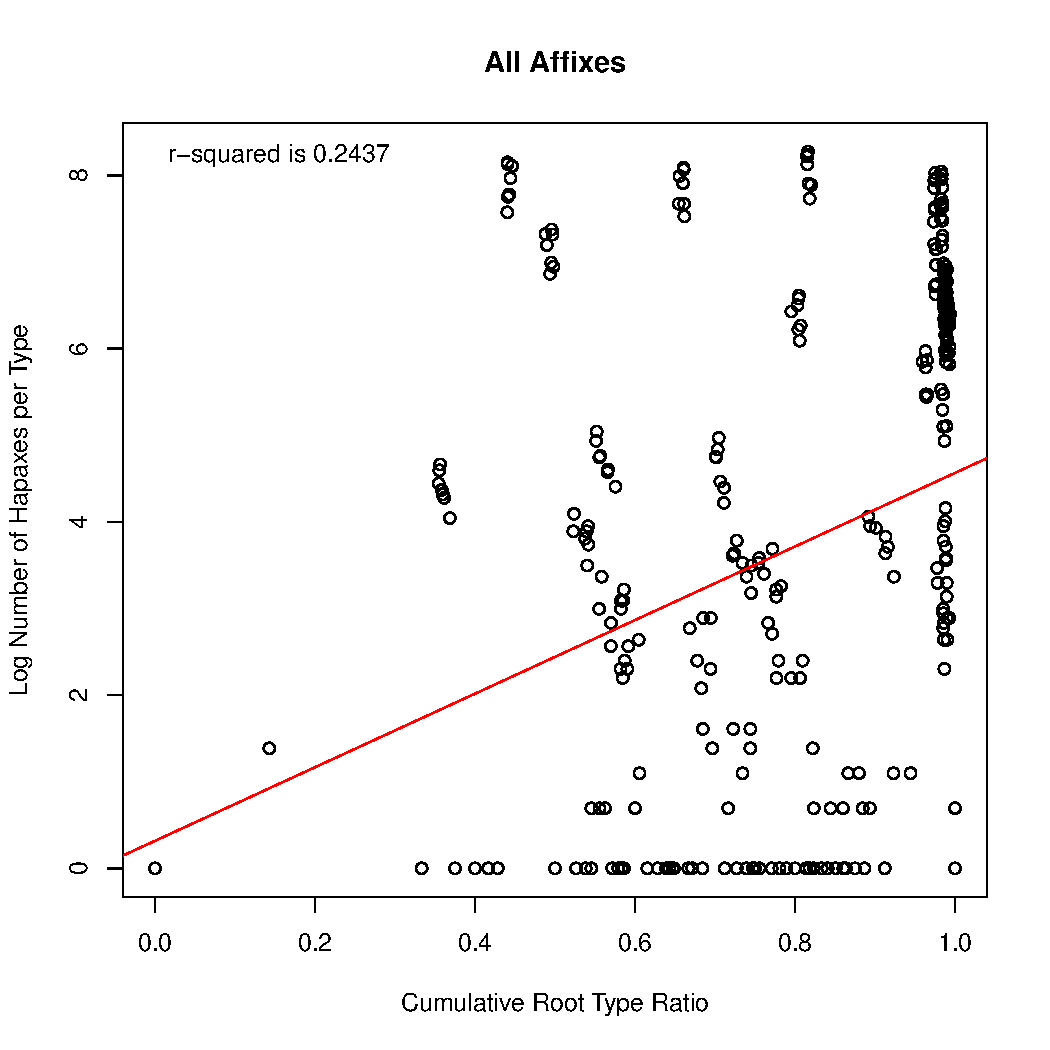
\includegraphics[width=\maxwidth]{figure/HapaxData-1} \caption[The Cumulative Root Frequency Ratio is positively correlated with the number of hapaxes in a non overlapping, but equal-sized subset of the corpus, r-squared = 0.2411, F(1,418) = 134.1, p less-than 2.2e16]{The Cumulative Root Frequency Ratio is positively correlated with the number of hapaxes in a non overlapping, but equal-sized subset of the corpus, r-squared = 0.2411, F(1,418) = 134.1, p less-than 2.2e16.}\label{fig:HapaxData}
\end{figure}

\begin{kframe}\begin{alltt}
\hlkwd{summary}\hlstd{(hd.mod1)}
\end{alltt}
\begin{verbatim}
## 
## Call:
## lm(formula = loghap ~ Ratio, data = Main)
## 
## Residuals:
##     Min      1Q  Median      3Q     Max 
## -4.5652 -1.8733 -0.3172  1.9643  5.9622 
## 
## Coefficients:
##             Estimate Std. Error t value Pr(>|t|)    
## (Intercept)   0.3172     0.2809   1.129     0.26    
## Ratio         4.2481     0.3643  11.662   <2e-16 ***
## ---
## Signif. codes:  0 '***' 0.001 '**' 0.01 '*' 0.05 '.' 0.1 ' ' 1
## 
## Residual standard error: 2.59 on 418 degrees of freedom
## Multiple R-squared:  0.2455,	Adjusted R-squared:  0.2437 
## F-statistic:   136 on 1 and 418 DF,  p-value: < 2.2e-16
\end{verbatim}
\end{kframe}
\end{knitrout}
\begin{knitrout}
\definecolor{shadecolor}{rgb}{0.969, 0.969, 0.969}\color{fgcolor}\begin{kframe}
\begin{alltt}
\hlkwd{rm}\hlstd{(}\hlkwc{list}\hlstd{=}\hlkwd{ls}\hlstd{())}
\hlkwd{setwd}\hlstd{(}\hlstr{'../Sources'}\hlstd{)}

\hlcom{# Read in kfolds data}
\hlstd{Main} \hlkwb{<-} \hlkwd{read.table}\hlstd{(}\hlstr{"kfolds_Redo"}\hlstd{,} \hlkwc{sep}\hlstd{=}\hlstr{"\textbackslash{}t"}\hlstd{,} \hlkwc{header}\hlstd{=}\hlnum{TRUE}\hlstd{)}

\hlcom{# Make it a dataframe}
\hlstd{Main} \hlkwb{<-} \hlkwd{data.frame}\hlstd{(Main)}

\hlcom{# Calculate Type Ratio}
\hlstd{Main} \hlkwb{<-} \hlkwd{transform}\hlstd{(Main,} \hlkwc{Ratio} \hlstd{= Above} \hlopt{/} \hlstd{Total)}

\hlcom{# Replace ones divided by zero with zero}
\hlstd{Main}\hlopt{$}\hlstd{Ratio[} \hlkwd{is.nan}\hlstd{( Main}\hlopt{$}\hlstd{Ratio ) ]} \hlkwb{<-} \hlnum{0}

\hlcom{# Convert the frequency counts to logarithmic scale}
\hlstd{Main}\hlopt{$}\hlstd{loghap} \hlkwb{<-} \hlkwd{log}\hlstd{(Main}\hlopt{$}\hlstd{Hapaxes)}

\hlcom{# Replace ones divided by zero with zero}
\hlstd{Main}\hlopt{$}\hlstd{loghap[} \hlkwd{is.nan}\hlstd{(Main}\hlopt{$}\hlstd{loghap ) ]} \hlkwb{<-} \hlnum{0}

\hlcom{# Replace negative values with zero}
\hlstd{Main}\hlopt{$}\hlstd{loghap[ Main}\hlopt{$}\hlstd{loghap} \hlopt{<} \hlnum{0} \hlstd{]} \hlkwb{<-} \hlnum{0}

\hlcom{# Ratio is the independant variable, and hapaxes are the dependent variable}
\hlkwd{plot}\hlstd{(loghap} \hlopt{~} \hlstd{Slope,} \hlkwc{data} \hlstd{= Main,}
  \hlkwc{xlim}\hlstd{=}\hlkwd{c}\hlstd{(}\hlnum{0}\hlstd{,} \hlnum{2}\hlstd{),}
  \hlkwc{ylim}\hlstd{=}\hlkwd{c}\hlstd{(}\hlnum{0}\hlstd{,} \hlnum{10}\hlstd{),}
  \hlkwc{xlab} \hlstd{=} \hlstr{"Cumulative Root Type Slope"}\hlstd{,}
  \hlkwc{ylab} \hlstd{=} \hlstr{"Log Number of Hapaxes per Type"}\hlstd{,}
  \hlkwc{main} \hlstd{=} \hlstr{"All Affixes"}
\hlstd{)}

\hlstd{hd.mod1} \hlkwb{=} \hlkwd{lm}\hlstd{(loghap} \hlopt{~} \hlstd{Slope,} \hlkwc{data} \hlstd{= Main)}

\hlkwd{abline}\hlstd{(fit} \hlkwb{<-} \hlkwd{lm}\hlstd{(loghap} \hlopt{~} \hlstd{Slope,} \hlkwc{data}\hlstd{=Main),} \hlkwc{col}\hlstd{=}\hlstr{'red'}\hlstd{)}
\hlkwd{legend}\hlstd{(}\hlstr{"topleft"}\hlstd{,} \hlkwc{bty}\hlstd{=}\hlstr{"n"}\hlstd{,} \hlkwc{legend}\hlstd{=}\hlkwd{paste}\hlstd{(}\hlstr{"r-squared is"}\hlstd{,}
  \hlkwd{format}\hlstd{(}\hlkwd{summary}\hlstd{(fit)}\hlopt{$}\hlstd{adj.r.squared,} \hlkwc{digits}\hlstd{=}\hlnum{4}\hlstd{)))}
\end{alltt}
\end{kframe}\begin{figure}
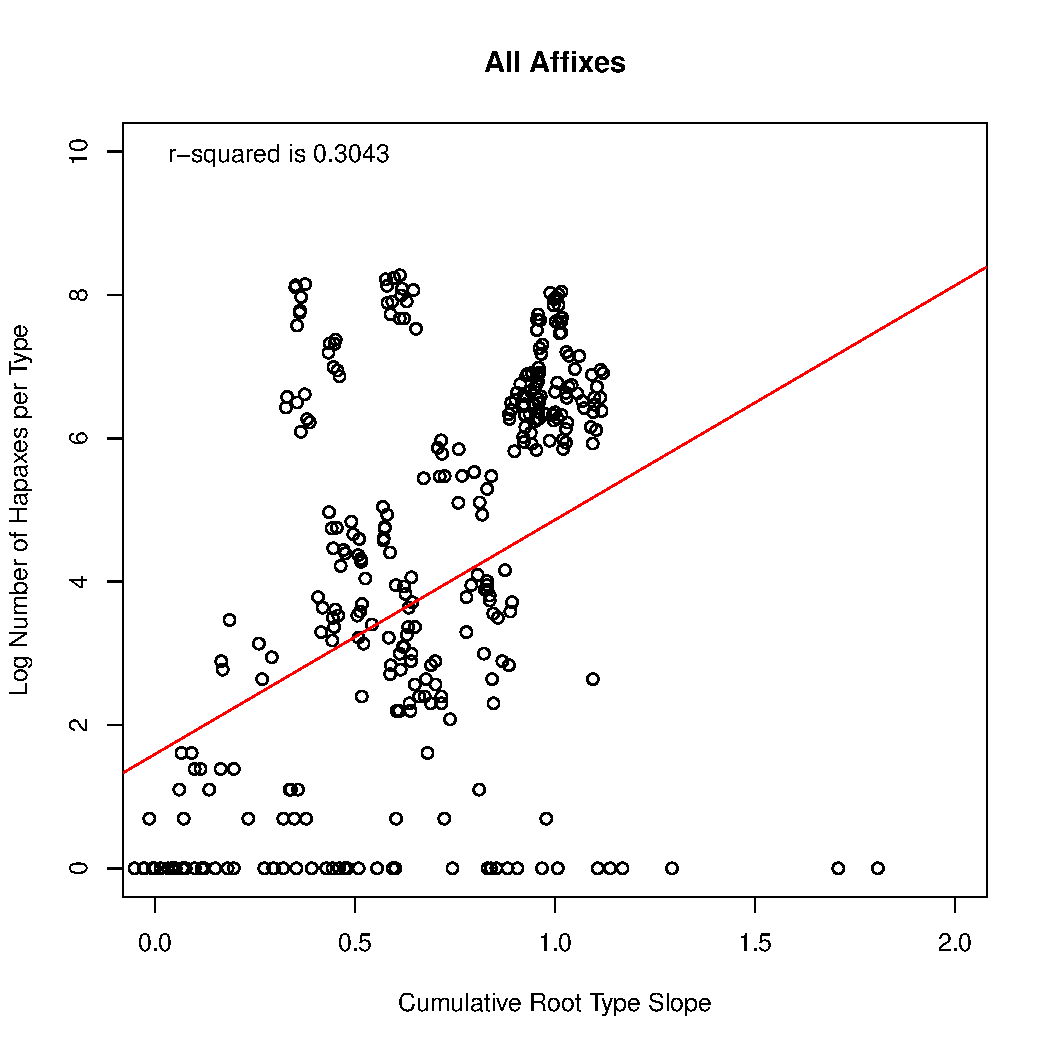
\includegraphics[width=\maxwidth]{figure/HapaxDataSlope-1} \caption[The Cumulative Root Frequency Ratio is positively correlated with the number of hapaxes in a non overlapping, but equal-sized subset of the corpus, r-squared = 0.2411, F(1,418) = 134.1, p less-than 2.2e16]{The Cumulative Root Frequency Ratio is positively correlated with the number of hapaxes in a non overlapping, but equal-sized subset of the corpus, r-squared = 0.2411, F(1,418) = 134.1, p less-than 2.2e16.}\label{fig:HapaxDataSlope}
\end{figure}

\begin{kframe}\begin{alltt}
\hlkwd{summary}\hlstd{(hd.mod1)}
\end{alltt}
\begin{verbatim}
## 
## Call:
## lm(formula = loghap ~ Slope, data = Main)
## 
## Residuals:
##      Min       1Q   Median       3Q      Max 
## -13.1634  -1.5930  -0.1624   1.6632   5.3915 
## 
## Coefficients:
##             Estimate Std. Error t value Pr(>|t|)    
## (Intercept)   1.5930     0.1747    9.12   <2e-16 ***
## Slope         3.2695     0.2423   13.49   <2e-16 ***
## ---
## Signif. codes:  0 '***' 0.001 '**' 0.01 '*' 0.05 '.' 0.1 ' ' 1
## 
## Residual standard error: 2.481 on 413 degrees of freedom
##   (5 observations deleted due to missingness)
## Multiple R-squared:  0.3059,	Adjusted R-squared:  0.3043 
## F-statistic:   182 on 1 and 413 DF,  p-value: < 2.2e-16
\end{verbatim}
\end{kframe}
\end{knitrout}

\begin{knitrout}
\definecolor{shadecolor}{rgb}{0.969, 0.969, 0.969}\color{fgcolor}\begin{kframe}
\begin{alltt}
\hlkwd{rm}\hlstd{(}\hlkwc{list}\hlstd{=}\hlkwd{ls}\hlstd{())}
\hlkwd{setwd}\hlstd{(}\hlstr{'../Sources'}\hlstd{)}

\hlcom{# Read in kfolds data}
\hlstd{Main} \hlkwb{<-} \hlkwd{read.table}\hlstd{(}\hlstr{"kfolds_Redo"}\hlstd{,} \hlkwc{sep}\hlstd{=}\hlstr{"\textbackslash{}t"}\hlstd{,} \hlkwc{header}\hlstd{=}\hlnum{TRUE}\hlstd{)}

\hlcom{# Make it a dataframe}
\hlstd{Main} \hlkwb{<-} \hlkwd{data.frame}\hlstd{(Main)}

\hlcom{# Calculate Type Ratio}
\hlstd{Main} \hlkwb{<-} \hlkwd{transform}\hlstd{(Main,} \hlkwc{Ratio} \hlstd{= Above} \hlopt{/} \hlstd{Total)}

\hlcom{# Replace ones divided by zero with zero}
\hlstd{Main}\hlopt{$}\hlstd{Ratio[} \hlkwd{is.nan}\hlstd{( Main}\hlopt{$}\hlstd{Ratio ) ]} \hlkwb{<-} \hlnum{0}

\hlcom{# Convert the frequency counts to logarithmic scale}
\hlstd{Main}\hlopt{$}\hlstd{loghap} \hlkwb{<-} \hlkwd{log}\hlstd{(Main}\hlopt{$}\hlstd{Hapaxes)}

\hlcom{# Replace ones divided by zero with zero}
\hlstd{Main}\hlopt{$}\hlstd{loghap[} \hlkwd{is.nan}\hlstd{(Main}\hlopt{$}\hlstd{loghap ) ]} \hlkwb{<-} \hlnum{0}

\hlcom{# Replace negative values with zero}
\hlstd{Main}\hlopt{$}\hlstd{loghap[ Main}\hlopt{$}\hlstd{loghap} \hlopt{<} \hlnum{0} \hlstd{]} \hlkwb{<-} \hlnum{0}

\hlcom{# Ratio is the independant variable, and hapaxes are the dependent variable}
\hlkwd{plot}\hlstd{(loghap} \hlopt{~} \hlstd{Yintercept,} \hlkwc{data} \hlstd{= Main,}
  \hlkwc{xlim}\hlstd{=}\hlkwd{c}\hlstd{(}\hlnum{0}\hlstd{,} \hlnum{2}\hlstd{),}
  \hlkwc{ylim}\hlstd{=}\hlkwd{c}\hlstd{(}\hlnum{0}\hlstd{,} \hlnum{10}\hlstd{),}
  \hlkwc{xlab} \hlstd{=} \hlstr{"Cumulative Root Type Y-Intercept"}\hlstd{,}
  \hlkwc{ylab} \hlstd{=} \hlstr{"Log Number of Hapaxes per Type"}\hlstd{,}
  \hlkwc{main} \hlstd{=} \hlstr{"All Affixes"}
\hlstd{)}

\hlstd{hd.mod1} \hlkwb{=} \hlkwd{lm}\hlstd{(loghap} \hlopt{~} \hlstd{Yintercept,} \hlkwc{data} \hlstd{= Main)}

\hlkwd{abline}\hlstd{(fit} \hlkwb{<-} \hlkwd{lm}\hlstd{(loghap} \hlopt{~} \hlstd{Ratio,} \hlkwc{data}\hlstd{=Main),} \hlkwc{col}\hlstd{=}\hlstr{'red'}\hlstd{)}
\hlkwd{legend}\hlstd{(}\hlstr{"topleft"}\hlstd{,} \hlkwc{bty}\hlstd{=}\hlstr{"n"}\hlstd{,} \hlkwc{legend}\hlstd{=}\hlkwd{paste}\hlstd{(}\hlstr{"r-squared is"}\hlstd{,}
  \hlkwd{format}\hlstd{(}\hlkwd{summary}\hlstd{(fit)}\hlopt{$}\hlstd{adj.r.squared,} \hlkwc{digits}\hlstd{=}\hlnum{4}\hlstd{)))}
\end{alltt}
\end{kframe}\begin{figure}
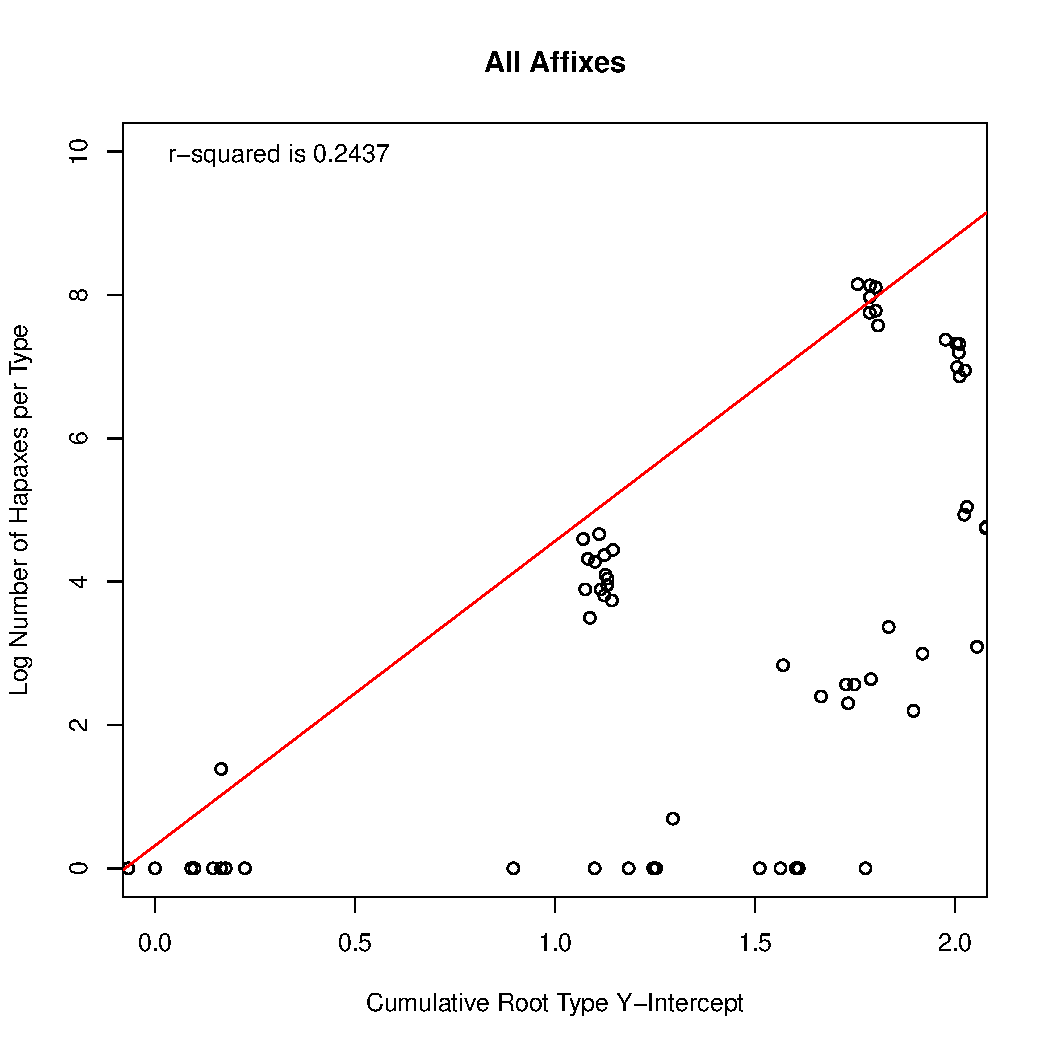
\includegraphics[width=\maxwidth]{figure/HapaxDataYintercept-1} \caption[The Cumulative Root Frequency Ratio is positively correlated with the number of hapaxes in a non overlapping, but equal-sized subset of the corpus, r-squared = 0.2411, F(1,418) = 134.1, p less-than 2.2e16]{The Cumulative Root Frequency Ratio is positively correlated with the number of hapaxes in a non overlapping, but equal-sized subset of the corpus, r-squared = 0.2411, F(1,418) = 134.1, p less-than 2.2e16.}\label{fig:HapaxDataYintercept}
\end{figure}

\begin{kframe}\begin{alltt}
\hlkwd{summary}\hlstd{(hd.mod1)}
\end{alltt}
\begin{verbatim}
## 
## Call:
## lm(formula = loghap ~ Yintercept, data = Main)
## 
## Residuals:
##     Min      1Q  Median      3Q     Max 
## -5.2869 -2.1718  0.0357  2.1746  5.8707 
## 
## Coefficients:
##             Estimate Std. Error t value Pr(>|t|)    
## (Intercept)  1.28985    0.25806   4.998 8.56e-07 ***
## Yintercept   0.56386    0.06249   9.023  < 2e-16 ***
## ---
## Signif. codes:  0 '***' 0.001 '**' 0.01 '*' 0.05 '.' 0.1 ' ' 1
## 
## Residual standard error: 2.722 on 413 degrees of freedom
##   (5 observations deleted due to missingness)
## Multiple R-squared:  0.1647,	Adjusted R-squared:  0.1627 
## F-statistic: 81.42 on 1 and 413 DF,  p-value: < 2.2e-16
\end{verbatim}
\end{kframe}
\end{knitrout}
For all 60 affixes, there is a significant correlation between Cumulative Root Frequency Ratio and the number of hapaxes of that type in non overalapping subsets. This correlation exists regardless of whether there the affix is verbal, or nominal, and derivational or inflectional. This indicates first, that in Swahili there is a correspondence between affixation and the type ratio, and furthermore, that the frequency of morphologically related competitors, and not the frequency of the bare stem, makes the correct prediction both in situations where a bare stem is possible, as well as situations where they are not.

This effect hold true when we evaluate the inflection affixes alone, as seen below, as well as for the derivational affixes alone.

\begin{knitrout}
\definecolor{shadecolor}{rgb}{0.969, 0.969, 0.969}\color{fgcolor}\begin{figure}
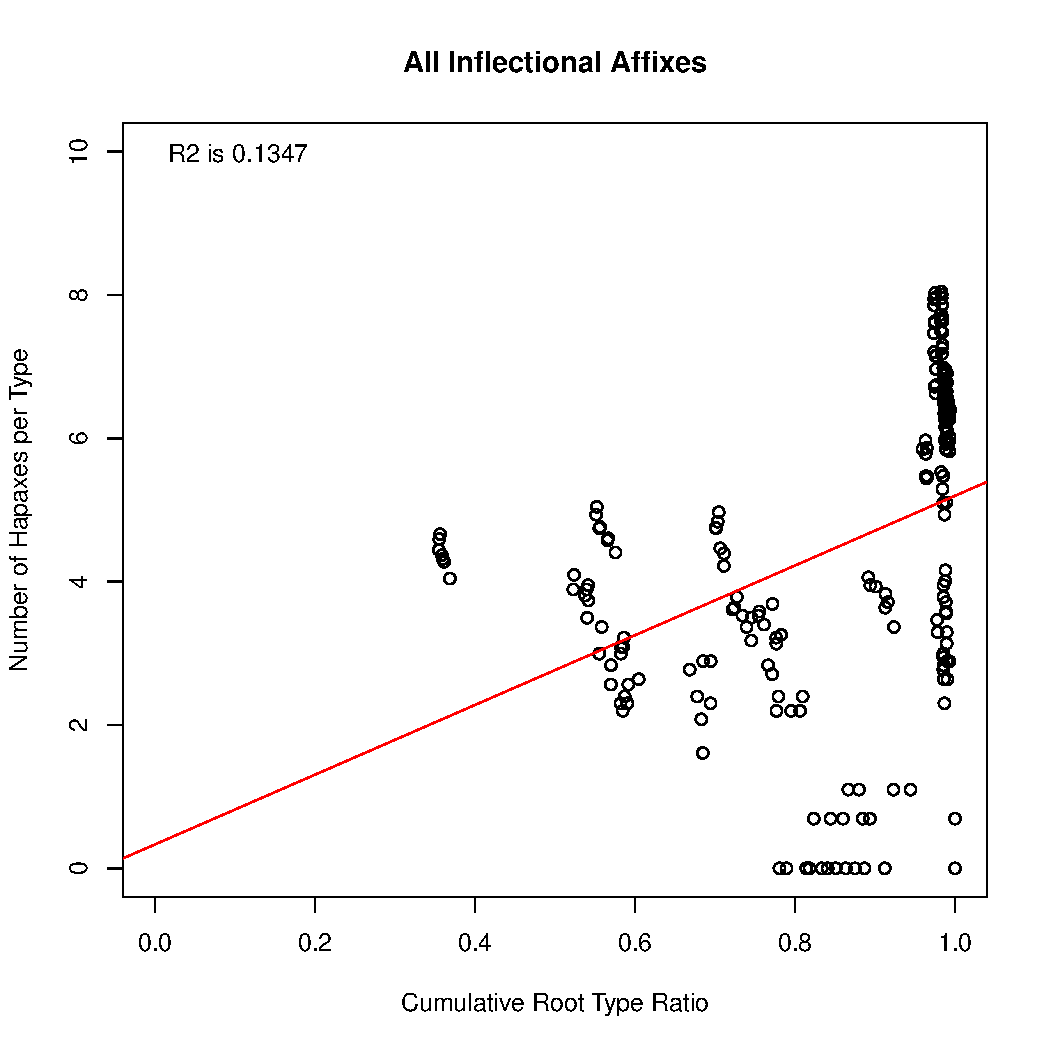
\includegraphics[width=\maxwidth]{figure/HapaxDataInflection-1} \caption[The Cumulative Root Frequency Ratio is positively correlated with the number of hapaxes in a non overlapping, but equal-sized subset of the corpus for all Inflection affixes, r-squared = 0.2632, F(1,236) = 85.65, p less-than 2.2e16]{The Cumulative Root Frequency Ratio is positively correlated with the number of hapaxes in a non overlapping, but equal-sized subset of the corpus for all Inflection affixes, r-squared = 0.2632, F(1,236) = 85.65, p less-than 2.2e16.}\label{fig:HapaxDataInflection}
\end{figure}

\begin{kframe}\begin{verbatim}
## 
## Call:
## lm(formula = loghap ~ Ratio, data = mdl1)
## 
## Residuals:
##     Min      1Q  Median      3Q     Max 
## -5.1980 -1.1352  0.7843  1.4935  2.9524 
## 
## Coefficients:
##             Estimate Std. Error t value Pr(>|t|)    
## (Intercept)   0.3337     0.6989   0.477    0.633    
## Ratio         4.8644     0.7902   6.156 3.18e-09 ***
## ---
## Signif. codes:  0 '***' 0.001 '**' 0.01 '*' 0.05 '.' 0.1 ' ' 1
## 
## Residual standard error: 2.101 on 236 degrees of freedom
## Multiple R-squared:  0.1383,	Adjusted R-squared:  0.1347 
## F-statistic: 37.89 on 1 and 236 DF,  p-value: 3.183e-09
\end{verbatim}
\end{kframe}
\end{knitrout}

\begin{knitrout}
\definecolor{shadecolor}{rgb}{0.969, 0.969, 0.969}\color{fgcolor}\begin{figure}
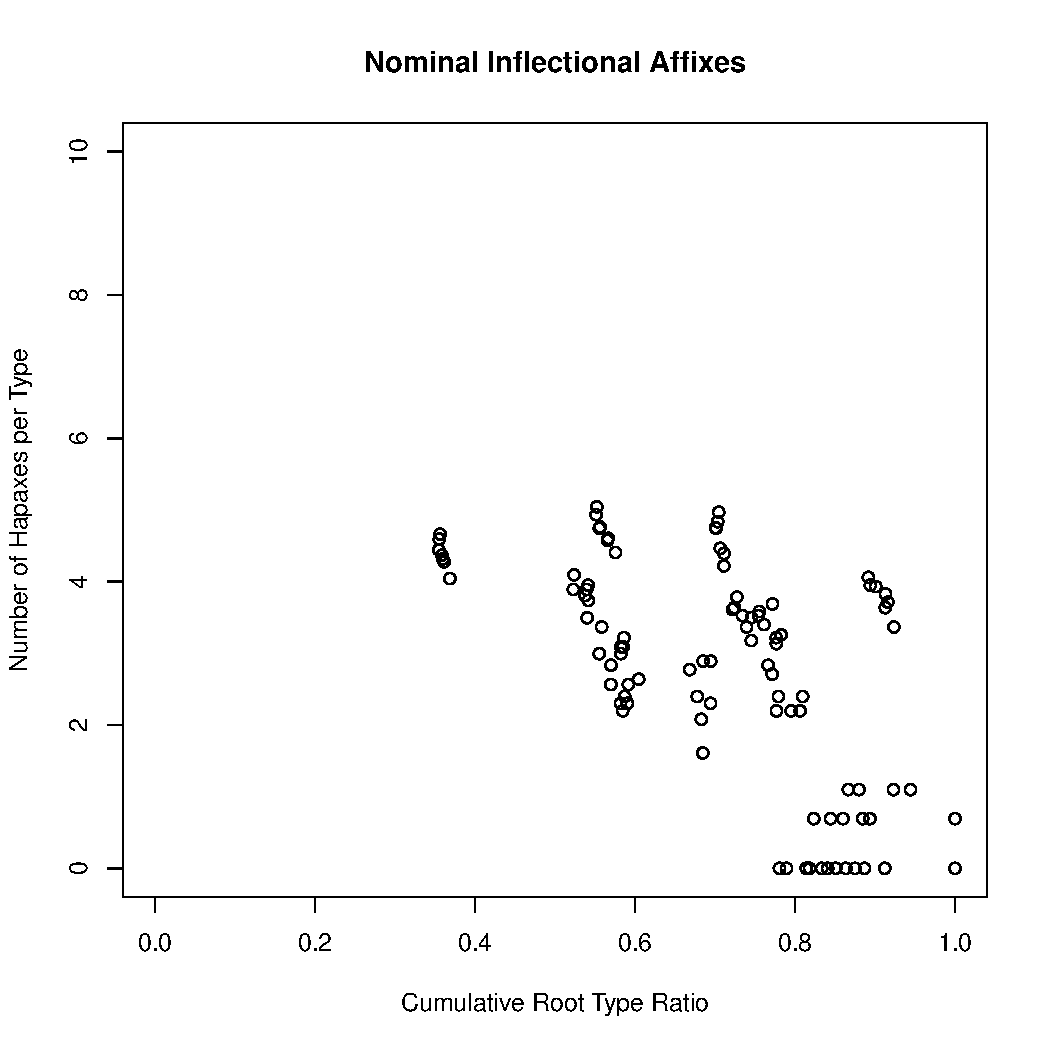
\includegraphics[width=\maxwidth]{figure/HapaxDataInflectionNom-1} \caption[The Cumulative Root Frequency Ratio is positively correlated with the number of hapaxes in a non overlapping, but equal-sized subset of the corpus for all Inflection affixes, r-squared = 0.2632, F(1,236) = 85.65, p less-than 2.2e16]{The Cumulative Root Frequency Ratio is positively correlated with the number of hapaxes in a non overlapping, but equal-sized subset of the corpus for all Inflection affixes, r-squared = 0.2632, F(1,236) = 85.65, p less-than 2.2e16.}\label{fig:HapaxDataInflectionNom}
\end{figure}

\begin{kframe}\begin{verbatim}
## 
## Call:
## lm(formula = loghap ~ Ratio, data = mdl1)
## 
## Residuals:
##     Min      1Q  Median      3Q     Max 
## -2.2644 -0.8711 -0.2033  0.9818  2.5020 
## 
## Coefficients:
##             Estimate Std. Error t value Pr(>|t|)    
## (Intercept)   7.2181     0.5313  13.586  < 2e-16 ***
## Ratio        -6.3470     0.7202  -8.813  3.2e-14 ***
## ---
## Signif. codes:  0 '***' 0.001 '**' 0.01 '*' 0.05 '.' 0.1 ' ' 1
## 
## Residual standard error: 1.227 on 103 degrees of freedom
## Multiple R-squared:  0.4299,	Adjusted R-squared:  0.4243 
## F-statistic: 77.66 on 1 and 103 DF,  p-value: 3.197e-14
\end{verbatim}
\end{kframe}
\end{knitrout}

\begin{knitrout}
\definecolor{shadecolor}{rgb}{0.969, 0.969, 0.969}\color{fgcolor}\begin{figure}
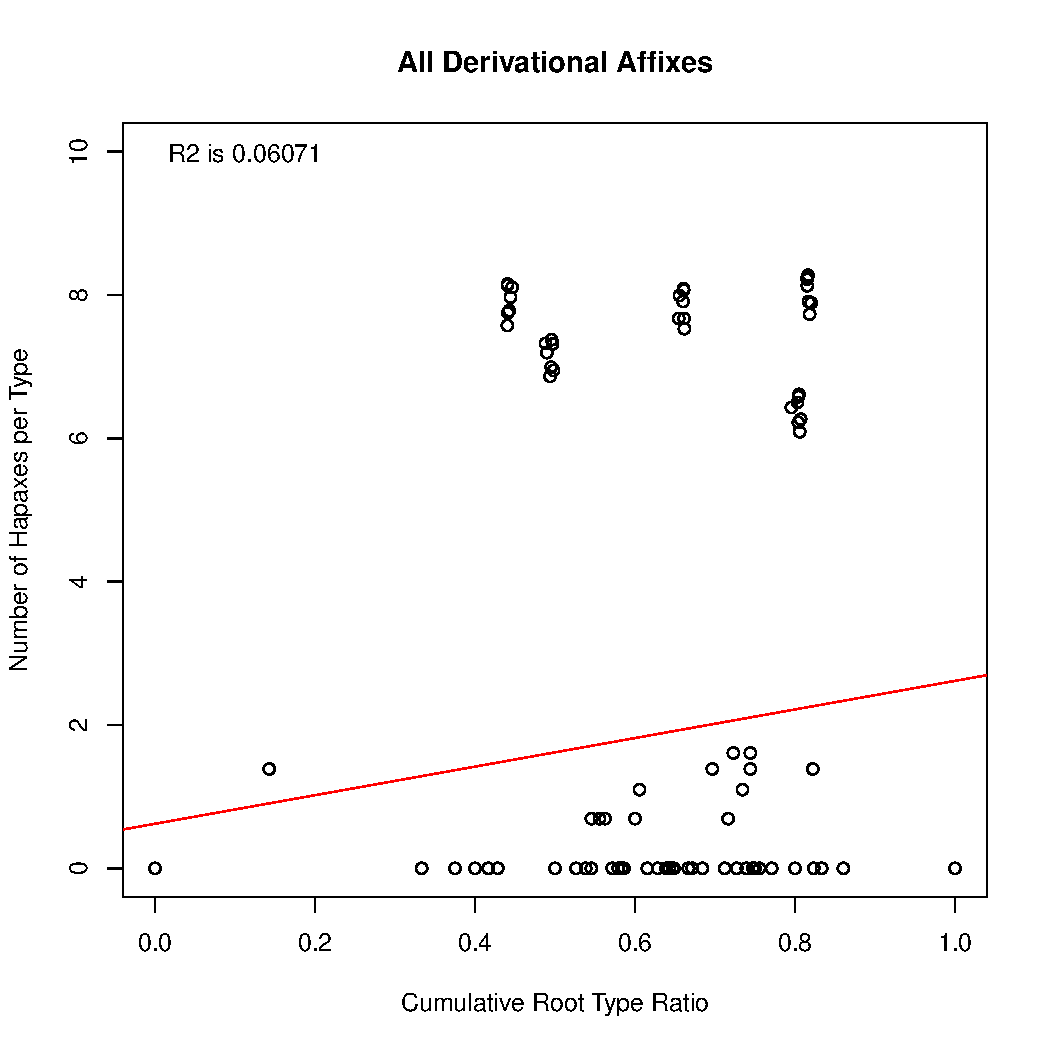
\includegraphics[width=\maxwidth]{figure/HapaxDataDerivation-1} \caption[The Cumulative Root Frequency Ratio is positively correlated with the number of hapaxes in a non overlapping, but equal-sized subset of the corpus for all Derivational affixes, r-squared = 0.04457, F(1,180) = 9.444, p less-than 0.002448]{The Cumulative Root Frequency Ratio is positively correlated with the number of hapaxes in a non overlapping, but equal-sized subset of the corpus for all Derivational affixes, r-squared = 0.04457, F(1,180) = 9.444, p less-than 0.002448}\label{fig:HapaxDataDerivation}
\end{figure}

\begin{kframe}\begin{verbatim}
## 
## Call:
## lm(formula = loghap ~ Ratio, data = mdl1)
## 
## Residuals:
##     Min      1Q  Median      3Q     Max 
## -2.6156 -1.8957 -0.6219 -0.6219  6.6507 
## 
## Coefficients:
##             Estimate Std. Error t value Pr(>|t|)    
## (Intercept)   0.6219     0.3307   1.881 0.061655 .  
## Ratio         1.9937     0.5595   3.563 0.000469 ***
## ---
## Signif. codes:  0 '***' 0.001 '**' 0.01 '*' 0.05 '.' 0.1 ' ' 1
## 
## Residual standard error: 2.849 on 180 degrees of freedom
## Multiple R-squared:  0.0659,	Adjusted R-squared:  0.06071 
## F-statistic:  12.7 on 1 and 180 DF,  p-value: 0.0004686
\end{verbatim}
\end{kframe}
\end{knitrout}

\begin{knitrout}
\definecolor{shadecolor}{rgb}{0.969, 0.969, 0.969}\color{fgcolor}\begin{figure}
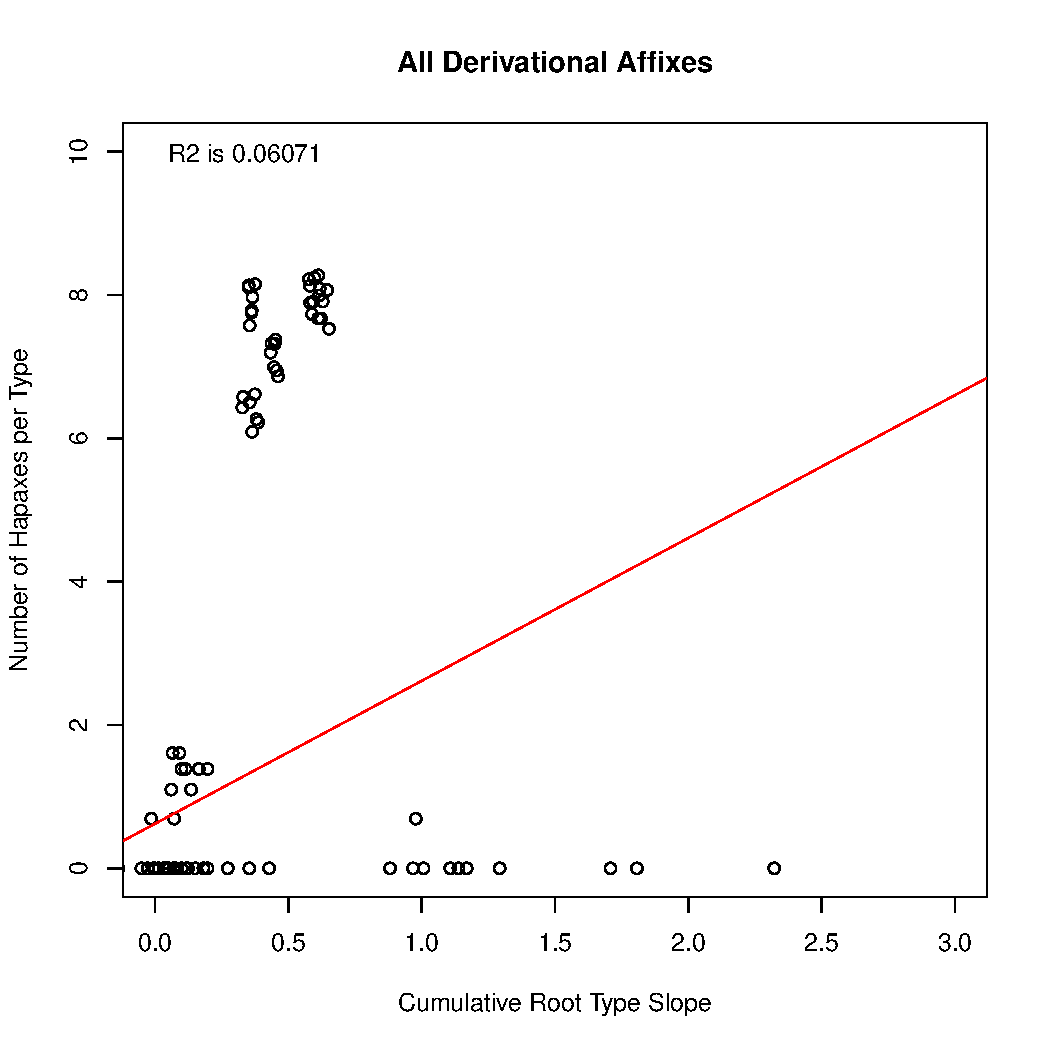
\includegraphics[width=\maxwidth]{figure/HapaxDataDerivationSlope-1} \caption[The Cumulative Root Frequency Ratio is positively correlated with the number of hapaxes in a non overlapping, but equal-sized subset of the corpus for all Derivational affixes, r-squared = 0.04457, F(1,180) = 9.444, p less-than 0.002448]{The Cumulative Root Frequency Ratio is positively correlated with the number of hapaxes in a non overlapping, but equal-sized subset of the corpus for all Derivational affixes, r-squared = 0.04457, F(1,180) = 9.444, p less-than 0.002448}\label{fig:HapaxDataDerivationSlope}
\end{figure}

\begin{kframe}\begin{verbatim}
## 
## Call:
## lm(formula = loghap ~ Slope, data = mdl1)
## 
## Residuals:
##    Min     1Q Median     3Q    Max 
## -5.996 -1.330 -1.330 -0.223  6.341 
## 
## Coefficients:
##             Estimate Std. Error t value Pr(>|t|)    
## (Intercept)   1.3298     0.2276   5.843 2.45e-08 ***
## Slope         1.3184     0.3808   3.463 0.000673 ***
## ---
## Signif. codes:  0 '***' 0.001 '**' 0.01 '*' 0.05 '.' 0.1 ' ' 1
## 
## Residual standard error: 2.882 on 175 degrees of freedom
##   (5 observations deleted due to missingness)
## Multiple R-squared:  0.06412,	Adjusted R-squared:  0.05877 
## F-statistic: 11.99 on 1 and 175 DF,  p-value: 0.0006726
\end{verbatim}
\end{kframe}
\end{knitrout}

\begin{knitrout}
\definecolor{shadecolor}{rgb}{0.969, 0.969, 0.969}\color{fgcolor}\begin{figure}
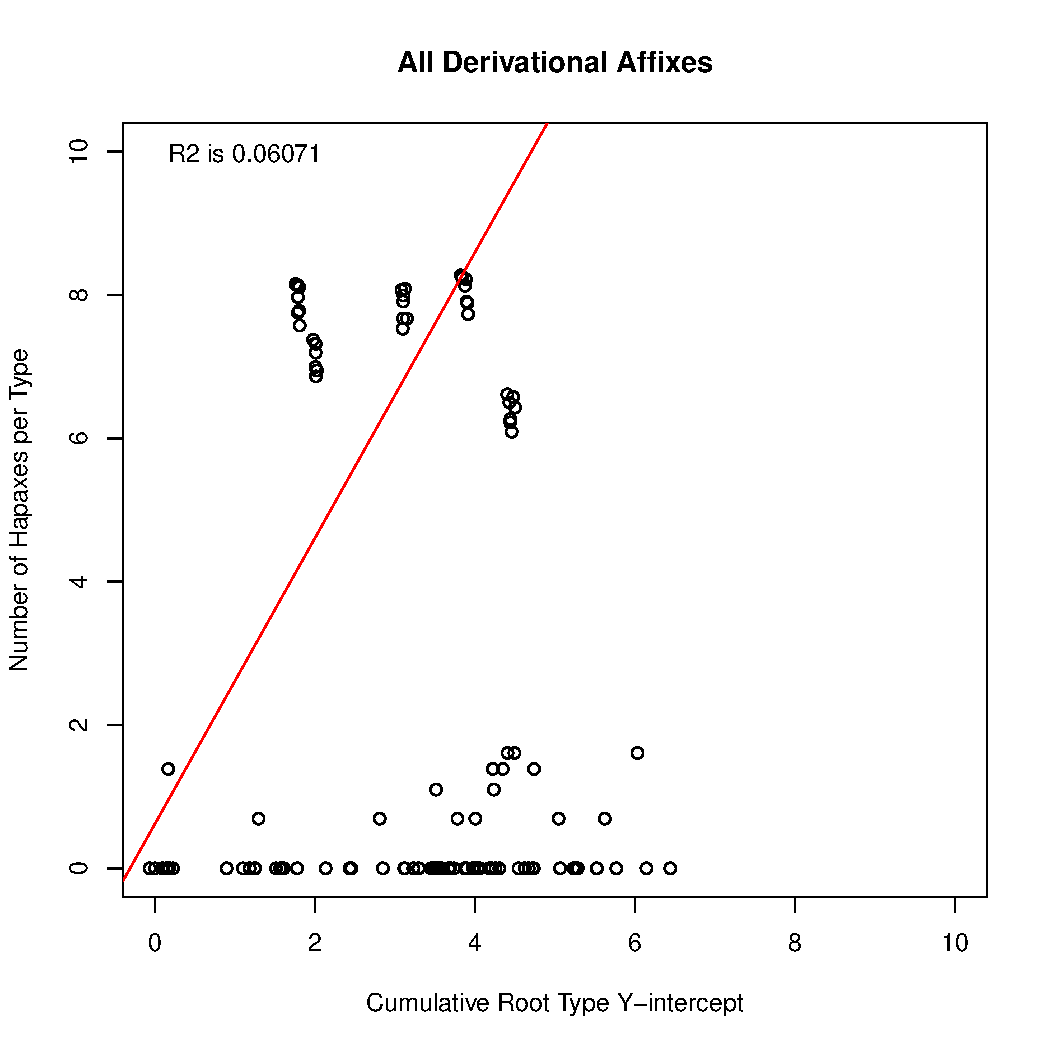
\includegraphics[width=\maxwidth]{figure/HapaxDataDerivationYintercept-1} \caption[The Cumulative Root Frequency Ratio is positively correlated with the number of hapaxes in a non overlapping, but equal-sized subset of the corpus for all Derivational affixes, r-squared = 0.04457, F(1,180) = 9.444, p less-than 0.002448]{The Cumulative Root Frequency Ratio is positively correlated with the number of hapaxes in a non overlapping, but equal-sized subset of the corpus for all Derivational affixes, r-squared = 0.04457, F(1,180) = 9.444, p less-than 0.002448}\label{fig:HapaxDataDerivationYintercept}
\end{figure}

\begin{kframe}\begin{verbatim}
## 
## Call:
## lm(formula = loghap ~ Yintercept, data = mdl1)
## 
## Residuals:
##     Min      1Q  Median      3Q     Max 
## -3.1187 -1.9535 -0.7814 -0.7814  6.7321 
## 
## Coefficients:
##             Estimate Std. Error t value Pr(>|t|)   
## (Intercept)   0.7814     0.3243   2.410  0.01700 * 
## Yintercept    0.3629     0.1105   3.285  0.00123 **
## ---
## Signif. codes:  0 '***' 0.001 '**' 0.01 '*' 0.05 '.' 0.1 ' ' 1
## 
## Residual standard error: 2.891 on 175 degrees of freedom
##   (5 observations deleted due to missingness)
## Multiple R-squared:  0.05809,	Adjusted R-squared:  0.0527 
## F-statistic: 10.79 on 1 and 175 DF,  p-value: 0.001231
\end{verbatim}
\end{kframe}
\end{knitrout}

\begin{knitrout}
\definecolor{shadecolor}{rgb}{0.969, 0.969, 0.969}\color{fgcolor}\begin{figure}
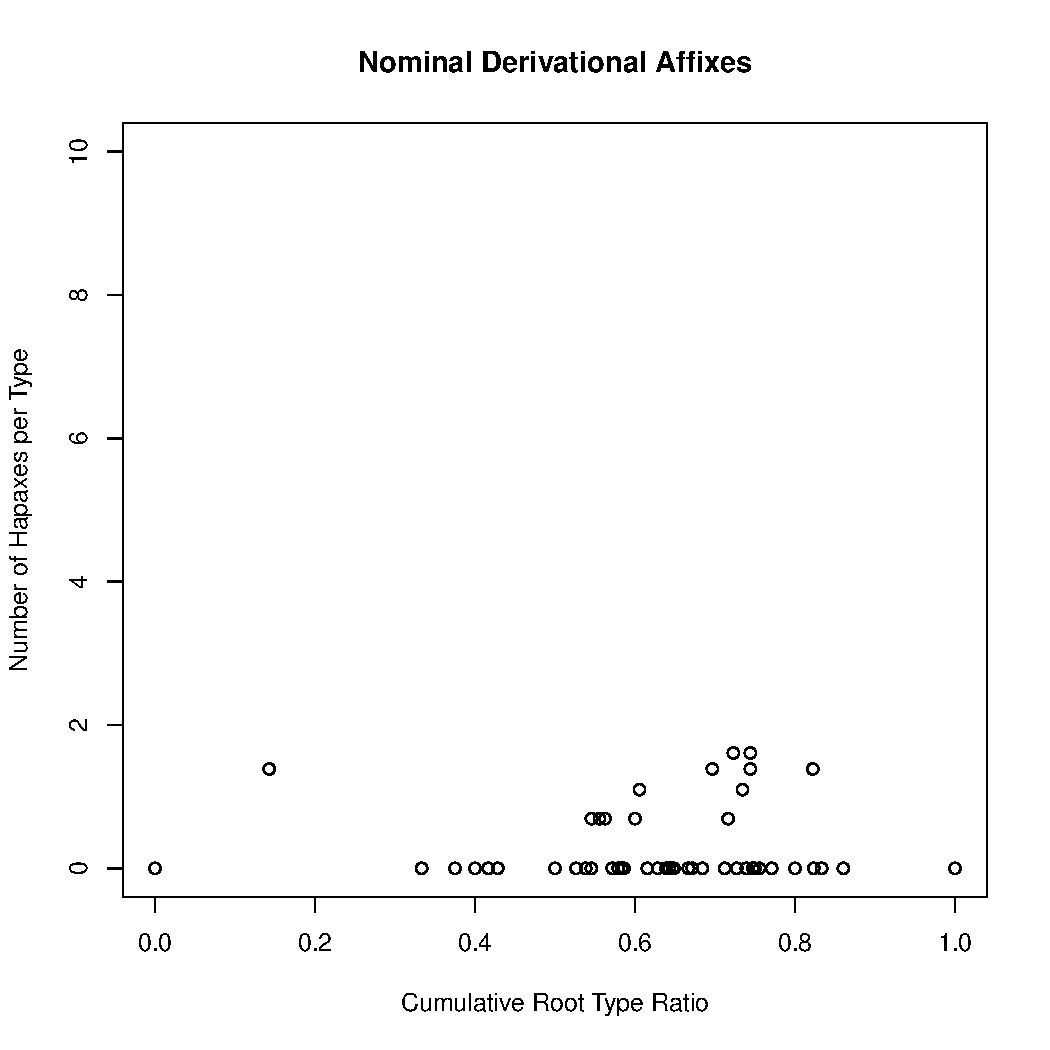
\includegraphics[width=\maxwidth]{figure/HapaxDataNomDerivation2-1} \caption[The Cumulative Root Frequency Ratio is positively correlated with the number of hapaxes in a non overlapping, but equal-sized subset of the corpus for Nominal Derivational affixes, r-squared = 0.05092, F(1,180) = 9.444, p less-than 0.0003]{The Cumulative Root Frequency Ratio is positively correlated with the number of hapaxes in a non overlapping, but equal-sized subset of the corpus for Nominal Derivational affixes, r-squared = 0.05092, F(1,180) = 9.444, p less-than 0.0003}\label{fig:HapaxDataNomDerivation2}
\end{figure}

\begin{kframe}\begin{verbatim}
## 
## Call:
## lm(formula = loghap ~ Ratio, data = mdl1)
## 
## Residuals:
##      Min       1Q   Median       3Q      Max 
## -0.21360 -0.16619 -0.04444 -0.04444  1.44271 
## 
## Coefficients:
##             Estimate Std. Error t value Pr(>|t|)  
## (Intercept)  0.04444    0.04180   1.063   0.2895  
## Ratio        0.16917    0.07292   2.320   0.0217 *
## ---
## Signif. codes:  0 '***' 0.001 '**' 0.01 '*' 0.05 '.' 0.1 ' ' 1
## 
## Residual standard error: 0.3541 on 145 degrees of freedom
## Multiple R-squared:  0.03578,	Adjusted R-squared:  0.02913 
## F-statistic: 5.381 on 1 and 145 DF,  p-value: 0.02175
\end{verbatim}
\end{kframe}
\end{knitrout}

\begin{knitrout}
\definecolor{shadecolor}{rgb}{0.969, 0.969, 0.969}\color{fgcolor}\begin{figure}
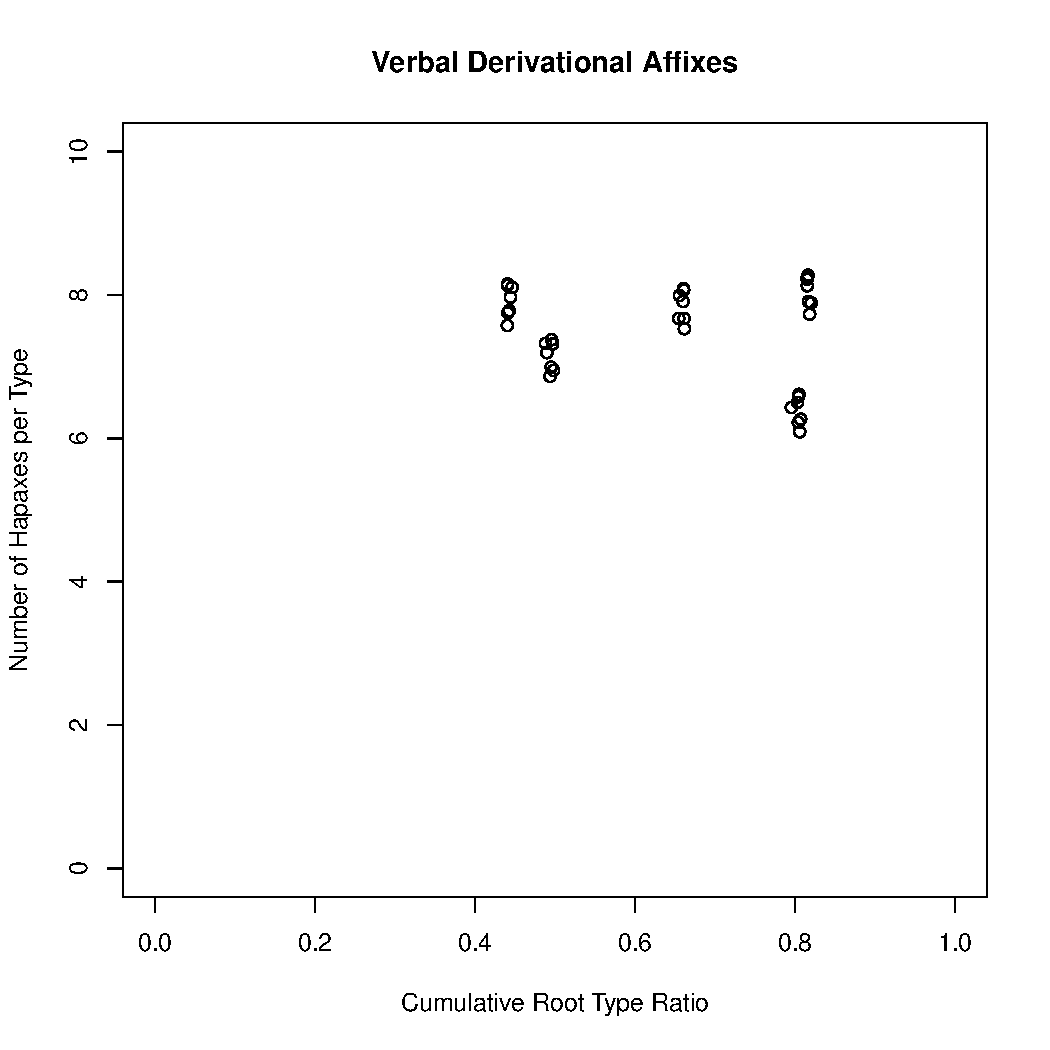
\includegraphics[width=\maxwidth]{figure/HapaxDataVerbalDerivation-1} \caption[The Cumulative Root Frequency Ratio is negatively correlated with the number of hapaxes in a non overlapping, but equal-sized subset of the corpus for Verbal Derivational affixes, r-squared = 0.1539, F(1,166) = 30.18, p less-than 0.000001]{The Cumulative Root Frequency Ratio is negatively correlated with the number of hapaxes in a non overlapping, but equal-sized subset of the corpus for Verbal Derivational affixes, r-squared = 0.1539, F(1,166) = 30.18, p less-than 0.000001}\label{fig:HapaxDataVerbalDerivation}
\end{figure}

\begin{kframe}\begin{verbatim}
## 
## Call:
## lm(formula = loghap ~ Ratio, data = mdl1)
## 
## Residuals:
##     Min      1Q  Median      3Q     Max 
## -1.2310 -0.6365  0.1245  0.5122  0.9621 
## 
## Coefficients:
##             Estimate Std. Error t value Pr(>|t|)    
## (Intercept)   8.0641     0.4801  16.795   <2e-16 ***
## Ratio        -0.9204     0.7260  -1.268    0.214    
## ---
## Signif. codes:  0 '***' 0.001 '**' 0.01 '*' 0.05 '.' 0.1 ' ' 1
## 
## Residual standard error: 0.6619 on 33 degrees of freedom
## Multiple R-squared:  0.04645,	Adjusted R-squared:  0.01756 
## F-statistic: 1.608 on 1 and 33 DF,  p-value: 0.2137
\end{verbatim}
\end{kframe}
\end{knitrout}
\section{Twitter Corpus}

Now that we've established a mechanism for predicting the production of novel types, we will expand the investigation to another corpus that will bolster these findings. Since we're using novelty as a means of identifying productivity, it's in our interest to establish true novelty, and not just an approximation of it. Ideally, one could elicit novel derived forms from speakers of Swahili by prompting them in a behavioral study. However, this sort of experiment would take a lot of work basically, and so another way to get there is to look at examples of words that we must assume to be productive uses given their content. Here, we make the assumption that novelty is associated not with hapaxes alone, but also with borrowed word forms that have recently occured. Fortunately, many Swahili speakers also speak English to various degrees, and not only that, but they choose to communicate with English and Swahili interchangeably on social media. Often, speakers will communicate in Swahili but will rely heavily on English borrowings when using open class word categories, which seems to be a thing in code switching (sources? theories? bleck). If speakers are incorporating English nominal and verbal borrowings into their language, and if we consider these instances to be examples of novel use, then we would consider the use of any examples of morphological marking to be examples of true novel use, and therefore productivity.

Given this, social media provides an opportunity to observe unprompted productivity in the wild. One platform that is particularly useful for these purposes is Twitter, for a few reasons. First, Twitter data is publicly available and there are a few interfaces that allow us to easily stream and save Tweets in real time. Second, we are able to filter these tweets based upon a few parameters that allow us to narrow the scope of inquiry. The most important of this is the geographic fiter that allows us to capture tweets written within a specific geographic area. For our purposes, this means that we can limit our range of tweets to include only those written in East Africa.

With there two parameters, we are able to filter out Tweets that are much less likely to contain languages other than Swahili and English. In order to further filter the data, we use a method of machine learning-based automatic language identification that allows us to pick individual 120 character tweets based upon their language. Given our empirical question about productivity, we want to find words that are recent borrowings in Swahili from English. Therefore, we want to identify tweets that contain both some degree of English, and some degree of Swahili. For our purposes, we'll label these tweets as code-switched tweets, and will tune our machine learning algorithm to identify tweets of this type. In the next section, we describe the development and creation of a corpus of code-switched tweets. In addition to these, we also create a corpus of Swahili tweets for comparison.

\subsection{Corpus Creation}

The aim of this section is to describe the development of a corpus using an automated mechanism of identifying the phenomenon of code-switching within a tweet. We define Code-Switching as the use of at least two separate languages within a single document. For the purposes of this study, the languages in question are Swahili and English, and the domain of inquiry is limited to twitter data originating from East Africa. Here, a single tweet constitutes a document, and therefore classification is binomial: Does a tweet contain CS or not?

\eq{
Herrera anajaribu stunts za Phelps
}

In order to perform this task, the system must correctly identify CS in documents containing phrases such as the one above. The example in (1) constitutes CS by virtue of the presence of multiple Swahili words, and that of an English common noun (i.e. \textit{stunts}). Crucially, the system must ignore proper nouns that may be borrowed from English or other languages  contains two proper nouns (i.e. \textit{Herrera} and \textit{Phelps}). This descrimintation task is performed using supervized learning, meaning  all tweets are labeled as either having CS or not in the training phase by hand. For a baseline, the machine then descriminates which prespecified features are associated with CS by means of the descriminitive learning algorithm of Logistic Regression. A second model  uses both English and Swahili classifiers to determine the count of Swahili and English words within a document. A judgement of whether CS occurs is then attested to whether or not both languages are detected within the same document.

\subsubsection{Methods}

As stated above, the task of CS identification is performed using supervised learning. Documents were collected using Twitter's streaming API to isolate geotagged tweets originating from the region of East Africa where Swahili is spoken both as a native language, and as an official language. These tweets were hand labeled as either English (0), Swahili (1), CS (2), or lacking any language/or having some third language (e.g. Portuguese)(3). For the current task, CS labels were altered to be positive (1) and all others were changed to negative (0). The training data contained 1,200 tweets balanced accross the 4 categories described above, and test contained a random sample of 100 tweets.

\subsubsection{Preprocessing}

The tweets were tokenized using a Twitter specific tokenizer, altered  from code made publicly available (). The tokenizer code was altered to extract and replace mentions (users mentioned within a tweet), hashtags (topics of discussion), and urls (weblinks provided within the tweet). These entities were replaced with variables denoting the entity type in order to preserve the fact that such entities were used in a tweet, but to also generalize across the usage of these entities. These entities were then effectively added or taken away from the model in the development stage in order to test whether their inclusion influenced performance.

\subsubsection{Feature Selection}

The primary feature used for language identification was character 5-grams and tokens as per the features used in previous studies \cite{tan14}. To extract 5-grams, a token is given a single start and 4 end symbols. The number of 5-grams extracted is exactly the number of characters in the token + 1, as in (2):

\eq{
\begin{tabular}[t]{lll}
  \textit{stunts} & $\rightarrow$ & [\^{}stun, stunt, tunts, unts\$, nts\$\$, ts\$\$\$, s\$\$\$\$] \\
\end{tabular}
}

Along with 5-grams, individual tokens, hashtags, mentions, and geotags were included as features. Features with a frequency count under a threshold of 10 were excluded, resulting in the use of around 22,000 features. Multiple generative, and descrimintative algorithms were tests, and finally Logistical Regression was decided upon as the best classifier (data included in coming section). The Logistical Regression algorithm was implemented usning the Scikit package for Python. The performance of the baseline model is discussed in the coming section.

\subsubsection{Voting Algorithm}
In addition to the baseline model, which simply learns the features associated with CS, a voting algorithm was created to improve performance. Rather than train on CS and non CS tweets as positive and negative examples, the voting algorithm employs two separate language classifiers of Swahili and English. Each classifier was trained on two 400,000 token corpora containing literature, and news sources. In addition, nearly 100,000 token corpora were employed to generate negative examples. The features used were character 5-grams, and tokens that occured above a frequency threshold of 10.

As opposed to the baseline model previously described, non-linguistic tokens were also excluded, in order to ensure unambiguously language specific features for each classifier. Furthermore, this model varied from the baseline by treating individual tokens as documents, rather than individual tweets. Judgements of the language of each subdocument (token) was performed based upon the features exctracted from them. Effectively, each classifier was run on each token's feature set. Each classifer labeled the subdocument as a positive or negative hit '0'. With a document, the positibe labels were then added to two separate lists (one for each language), and the totals were compared. If both classifiers returned a non-empty set, then the tweet was labeled as CS. That is, if at least one token was identified as Swahili, and at least one token was identified as English, then it was considered CS. The coming section compares the results of the baseline and voting models.

\subsubsection{Results}

Table 1 outlines the ablation of features used in the baseline model. Clearly, the inculsion of Twitter specific features enhances the ability of the model to predict CS. However, geotags, which could conceivably help the model if users in certain say urban areas were more likely to use CS, were unaffective. Oddly, the inclusion of geotags hinders accuracy, but boosts the F1 score. As a result of the experiment in Table 1, the features used were: character 5-grams, tokens, mentions, hashtags

\begin{table}[h]
\caption{Feature use in Perceptron Algorithm}
\centering
\begin{tabular}{llllll}
\cline{2-6}
  & \textbf{Accuracy} & \textbf{Precision} & \textbf{Recall} &
                                                               \textbf{F1 Score} & \textbf{Features}          \\ \cline{2-6} 
1 & 65.00\%     & 0.4977             & 0.4944          & 0.4631            & \textit{Character 5-grams} \\ \cline{2-6} 
2 & 74.00\%     & 0.5000             & 0.500           & 0.4902            & \textit{Previous+Tokens}   \\ \cline{2-6} 
3 & 68.00\%     & 0.5050             & 0.5111          & 0.4802            & \textit{Previous+Mentions} \\ \cline{2-6} 
4 & 78.00\%     & 0.5159             & 0.5222          & 0.5137            & \textit{Previous+Hashtags} \\ \cline{2-6} 
5 & 76.00\%     & 0.5312             & 0.5556          & 0.5294            & \textit{Previous+Geotags} 
\end{tabular}
\end{table}

After isolating the highest performing feature set, both generative (Naive Bayes) and descriminative algorthims ( Perceptron and Logistic Regression) were compared to isolate the best performance. Table 2 demonstrates that Logistic Regresson outperforms the other algorthims to a high degree, and so this algorithm is used in the baseline model.

\begin{table}[h]
\caption{Best Models using Various Algorithms}
\centering
\begin{tabular}{llllll}
\cline{2-6}
  & \textbf{Accuracy} & \textbf{Precision} & \textbf{Recall} & \textbf{F1 Score} & \textbf{Algorithm}               \\ \cline{2-6} 
1 & 76.00\%           & 0.5312             & 0.5294          & 0.5294            & \textit{Multinomial Naive Bayes} \\ \cline{2-6} 
2 & 78.00\%           & 0.4977             & 0.4944          & 0.4631            & \textit{Perceptron}              \\ \cline{2-6} 
3 & 89.00\%           & 0.6893             & 0.6722          & 0.6801            & \textit{Logistic Regression}     \\ \cline{2-6} 
\end{tabular}
\end{table}

The highest performance of the baseline model is \%89.00 accuracy, with an F1 score of 0.6801 (line 3: Table 2). To improve on this, the voting model was developed. Before creating such a model however, each the highest performing baseline model was tested on each language available in training. This test can show us how well the model descriminates individual languages for consideration in the voting model. Table 3 shows that the model's performance is indirectly propostional to the amount of English used in a tweet in a scalar manner.

\begin{table}[h]
\caption{Best Model + Algorithm detecting various Languages}
\centering
\begin{tabular}{llllll}
\cline{2-6}
  & \textbf{Accuracy} & \textbf{Precision} & \textbf{Recall} & \textbf{F1 Score} & \textbf{Language}       \\ \cline{2-6} 
1 & 80.00\%           & 0.7849             & 0.8128          & 0.5294            & \textit{English}        \\ \cline{2-6} 
2 & 89.00\%           & 0.6893             & 0.6722          & 0.6801            & \textit{Code Switching} \\ \cline{2-6} 
3 & 93.00\%           & 0.8114             & 0.7833          & 0.7965            & \textit{Swahili}        \\ \cline{2-6} 
\end{tabular}
\end{table}

Whereas Swahili has a rather high performance (\%93.00 accuracy, 0.7965 F1), CS (\%89.00 accuracy, 0.6801 F1), and English (\%80.00 accuracy, 0.52945 F1) fall behind. Based upon the evidence in Table 3, one could ascribe a weight of higher confidence to the detection of Swahili than English in the voting algorithm, however performance was not influenced by weighting. The results of the voting model are shown in Table 4.

\begin{table}[h]
\caption{Baseline versus Voting Model}
\centering
\begin{tabular}{llllll}
\cline{2-6}
  & \textbf{Accuracy} & \textbf{Precision} & \textbf{Recall} & \textbf{F1 Score} & \textbf{Model}       \\ \cline{2-6} 
1 & 89.00\%           & 0. 6893             & 0.6722          & 0.6801            & \textit{Baseline}        \\ \cline{2-6} 
2 & 90.00\%           & 0.4500             & 0.5000          & 0.4737
                                                                                 & \textit{Voting Model} \\ \cline{2-6} 
\end{tabular}
\end{table}

The voting algorithm did outperform the baseline model in accuracy, but the F1 score was much lower. This lower score can be ascribed to the fact that the number of (sub)documents is much larger, and that two different classifiers (as opposed to only one) were implemented in the descrimintation task. The results are further discussed in the next section.

\subsubsection{Discussion}

The data show that CS can be detected to a high degree of accuracy given the very low number of training examples and the high performance. It may be the case that increasing the size of training and test examples would increase baseline performance. Furthermore, rather than using news and literature sources as training data in the voting model, using Tweets in each language should increase the model given that that domain of usage is quite different indeed. For the low performance in English in general, I propose that sociolinguistic factors impact the outcomes. Specifically, a cursory looks at the data reveal that people in East Africa tend use text speak in English much more than in Swahili. That is, shortened and novel linguistic forms may be used more often by those who tweet in English rather than Swahili. More concretely, Swahili does not seem to have many examples of altered spelling (e.g. 'c u' for 'see you') or acronyms (e.g. lol for 'laugh out loud'). This sort of difference is unavoidable, and just a consequence of the data.

The overall application in detecting CS is to give insight into the world of language change in the realm of Linguistics, and can additionally have application other NLP tasks (e.g. relation extraction) where CS is common. As performance increases so can the confidence in building a corpors for more detailed analyses of language interaction along with the ability to accurately implement other language applications. Having already collected up to 1 million tweets over time, the highest performing algortihm will be applied to these tweets to generate an openly available corpus of CS collapsing across users. In the future, this project aim to track conversations between individual to ask more discourse oriented questions about code-switching. In theory, the techniques described here can be used in any set of languages to generate corpora of languages where CS is common.

\subsection{Applying the Algorithm to the Corpus}

This part is still to be done. I had done it previously, but have since collected more data, and need to reanalyze.

\subsection{Twitter Corpus Analysis}

Here, I'll take the ratios from the original study and compare them to codeswitched examples, and hapax counts.


\bibliographystyle{lsalike}
\par\bigskip
\bibliography{diss}

\end{document}
